\documentclass[a4paper,10pt]{report}
\usepackage[utf8x]{inputenc}
\usepackage[T1]{fontenc}
\usepackage[a4paper, margin=3cm]{geometry}

% Load ``float'' before ``hyperref`` before ''algorithm``
% Note: ''algorithm`` would load ''float`` by itself
\usepackage{appendix}
\usepackage{longtable}
\usepackage[nonumberlist,acronym]{glossaries}

\usepackage{float}


\usepackage{amsmath}
\usepackage{amssymb}
\usepackage{amsfonts}
\usepackage{amsopn}
\usepackage{braket}
\usepackage{bbm}
\usepackage{dsfont}
% \usepackage{mathabx}


% Various new commands that ease typesetting math even further
% \newcommand{\assign}{\ensuremath{\coloneq}}
% \newcommand{\rassign}{\ensuremath{\eqcolon}}
\newcommand{\assign}{\ensuremath{:=}}
\newcommand{\rassign}{\ensuremath{=:}}
\newcommand{\seteq}{\ensuremath{\overset{!}{=}}}

\newcommand{\of}[1]{\ensuremath{\left( #1 \right)}}
\newcommand{\ofs}[1]{\ensuremath{\left( #1 \right)}}

\newcommand{\norm}[1]{\ensuremath{\| #1 \|}}

\newcommand{\tmop}[1]{\ensuremath{\operatorname{#1}}}

\newcommand{\id}{\ensuremath{\mathds{1}}}
% \newcommand{\id}{\ensuremath{I}}

\newcommand{\kron}[1]{\ensuremath{\delta_{#1}}}

\newcommand{\conj}[1]{\ensuremath{\overline{#1}}}

\newcommand{\inv}{\ensuremath{{}^{-1}}}
\newcommand{\T}{\ensuremath{{}^{\textnormal{T}}}}
\newcommand{\herm}{\ensuremath{{}^{\textnormal{H}}}}

\newcommand{\tr}{\ensuremath{\textnormal{Tr}}}

\newcommand{\ft}[1]{\ensuremath{\mathcal{F}\left(#1\right)}}
\newcommand{\ift}[1]{\ensuremath{\mathcal{F}^{-1}\left(#1\right)}}

\newcommand{\fft}[1]{\ensuremath{\mathtt{FFT}\left(#1\right)}}
\newcommand{\ifft}[1]{\ensuremath{\mathtt{IFFT}\left(#1\right)}}

\newcommand{\dotp}[2]{\ensuremath{\langle #1 , #2 \rangle}}
\renewcommand{\braket}[1]{\ensuremath{\left\langle #1 \right\rangle}}

\newcommand{\bigO}[1]{\ensuremath{\mathcal{O}\left( #1 \right)}}

\newcommand{\laplace}{\ensuremath{\operatorname{\Delta}}}

\newcommand{\di}[1]{\ensuremath{\mathrm{d}#1}}
\newcommand{\diff}[3][]{\frac{\mathrm{d}^{#1}#2}{\mathrm{d}#3^{#1}}}
\newcommand{\pdiff}[2]{\frac{\partial #1}{\partial #2}}
%\newcommand{\pdiff}[3][]{\frac{\partial^{#1}#2}{\partial #3^{#1}}}
%\newcommand{\pdiffn}[3]{\frac{\partial^{#1}#2}{\partial #3^{#1}}}
% EOF

\usepackage{graphicx}
\usepackage{subfig}
\usepackage{asymptote}
\usepackage{tikz}

\usepackage[chapter]{algorithm}
\usepackage{algorithmic}

\usepackage{color}
\usepackage{relsize}
\usepackage[scaled=0.8]{beramono}
\usepackage{listings}

\definecolor{gray}{gray}{0.55}

% Python Code macro ------------------------------------------------------------

\newcommand{\python}[1] {
  \lstset{language=python,
          basicstyle=\smaller,
          basewidth=0.58em,
          columns=fixed,
          tabsize=2,
          fontadjust=true,
          frame=l,
          xleftmargin=4.2pt,
          numbers=left,
          stepnumber=2,
          breaklines=true,
          breakindent=0pt,
          prebreak=\mbox{\tiny$\searrow$},
          postbreak=\mbox{{\color{gray}$\cdots$}},
          keywordstyle=\bfseries,
          keywords={access,and,break,class,continue,def,del,elif ,else,
          except,exec,finally,for,from,global,if,import,in,is,
          lambda,not,or,pass,print,raise,return,try,while,
          True, False, None, self, from, import, as},
          numberstyle=\color{gray},
          commentstyle=\color{gray},
          stringstyle=\textit,
          showstringspaces=false,
        }
  \lstinputlisting{#1}
}

% C++ Code macro ---------------------------------------------------------------

\newcommand{\cpp}[1] {
  \lstset{language=c++,
          basicstyle=\smaller,
          basewidth=0.58em,
          columns=fixed,
          tabsize=2,
          fontadjust=true,
          frame=l,
          xleftmargin=4.2pt,
          numbers=left,
          stepnumber=2,
          breaklines=true,
          breakindent=0pt,
          prebreak=\mbox{\tiny$\searrow$},
          postbreak=\mbox{{\color{gray}$\cdots$}},
          numberstyle=\color{gray},
          commentstyle=\color{gray},
          stringstyle=\textit,
          showstringspaces=false,
        }
  \lstinputlisting{#1}
}

% Gnu R Code macro -------------------------------------------------------------

\newcommand{\gnuR}[1] {
  \lstset{language=R,
          basicstyle=\smaller,
          basewidth=0.58em,
          columns=fixed,
          tabsize=2,
          fontadjust=true,
          frame=l,
          xleftmargin=4.2pt,
          numbers=left,
          stepnumber=2,
          numberstyle=\color{gray},
          commentstyle=\color{gray},
          stringstyle=\textit,
          showstringspaces=false,
          literate={<-}{{$\leftarrow$}}1 {~}{{$\sim$}}1,
          escapeinside={(*}{*)}
        }
  \lstinputlisting{#1}
}



\usepackage{url}
\usepackage{placeins}
\usepackage{microtype}

% Design of chapter pages
\usepackage[Lenny]{fncychap}

% Links in pdf
\usepackage{color}
\newcommand{\blue}{ \color{blue} }
\definecolor{linkcol}{rgb}{0,0,0.4}
\definecolor{citecol}{rgb}{0.5,0,0}

\usepackage[pagebackref,hyperindex=true]{hyperref}
\hypersetup
{
colorlinks=true,
linkcolor=linkcol,
citecolor=citecol,
urlcolor=linkcol
}




% nicer backref links
\renewcommand*{\backref}[1]{}
\renewcommand*{\backrefalt}[4]{%
\ifcase #1 %
(Not cited.)%
\or
(Cited on page~#2.)%
\else
(Cited on pages~#2.)%
\fi}
\renewcommand*{\backrefsep}{, }
\renewcommand*{\backreftwosep}{ and~}
\renewcommand*{\backreflastsep}{ and~}

\parindent 0cm

\newcommand{\clearemptydoublepage}{\newpage{\pagestyle{empty}\cleardoublepage}}

\newcommand{\circnum}[1]{\mbox{\textcircled{\tiny #1}}}%

\newglossary{abbrev}{abs}{abo}{List of Abbreviations}
\newglossaryentry{IRLS}{
  name        = IRLS ,
  description = iteratively reweighted least squares ,
  type        = abbrev
}
\newglossaryentry{PRPT}{
  name        = PRPT ,
  description = proximal point ,
  type        = abbrev
}
\newglossaryentry{DTI}{
  name        = DTI ,
  description = diffusion tensor imaging ,
  type        = abbrev
}
\newglossaryentry{CT}{
  name        = CT ,
  description = computer tomography ,
  type        = abbrev
}
\newglossaryentry{BLAS}{
  name        = BLAS ,
  description = basic linear algebra subprograms ,
  type        = abbrev
}
\newglossaryentry{DT-MRI}{
  name        = DTMRI ,
  description = diffusion tensor magnetic resonance imaging ,
  type        = abbrev
}
\newglossaryentry{MRI}{
  name        = MRI ,
  description = magnetic resonance imaging ,
  type        = abbrev
}
\newglossaryentry{VPP}{
  name        = VPP ,
  description = Video++ ,
  type        = abbrev
}
\newglossaryentry{TV}{
  name        = TV ,
  description = total variation ,
  type        = abbrev
}
\newglossaryentry{MTVMTL}{
  name        = MTVMTL ,
  description = Manifold total variation minimization library ,
  type        = abbrev
}
\newglossaryentry{OMP}{
  name        = OMP ,
  description = OpenMP ,
  type        = abbrev
}
\newglossaryentry{SIMD}{
  name        = SIMD ,
  description = single instruction multiple data ,
  type        = abbrev
}
\newglossaryentry{SSE}{
  name        = SSE ,
  description = streaming SIMD extensions ,
  type        = abbrev
}
\newglossaryentry{AVX}{
  name        = AVX ,
  description = advanced vector extensions ,
  type        = abbrev
}
\newglossaryentry{SPD}{
  name        = SPD ,
  description = symmetric positive definite ,
  type        = abbrev
}
\newglossaryentry{SO}{
  name        = SO ,
  description = special orthogonal ,
  type        = abbrev
}
\newglossaryentry{OpenGL}{
  name        = OpenGL ,
  description = open graphics library ,
  type        = abbrev
}
\newglossaryentry{OpenCV}{
  name        = OpenCV ,
  description = open computer vision ,
  type        = abbrev
}
\newglossaryentry{GLUT}{
  name        = GLUT ,
  description = OpenGL utility toolkit ,
  type        = abbrev
}
\newglossaryentry{GLEW}{
  name        = GLEW ,
  description = OpenGL extension wrangler library ,
  type        = abbrev
}
\newglossaryentry{CGAL}{
  name        = CGAL ,
  description = computational geometry algorithms library ,
  type        = abbrev
}
%\newglossaryentry{CBR}{
%  name        = CBR ,
%  description = chromaticity-brightness ,
%  type        = abbrev
%}
\makenoidxglossaries

\begin{document}

\begin{titlepage}
\begin{center}
  \hfill
  \vspace{2.0cm}

  { \huge\textsc{\LARGE A fast C++ Template library for Total Variation Minimization of manifold-valued 
  two- and three-dimensional images\\[10pt]
  }}
  	~\\[20pt]
	
   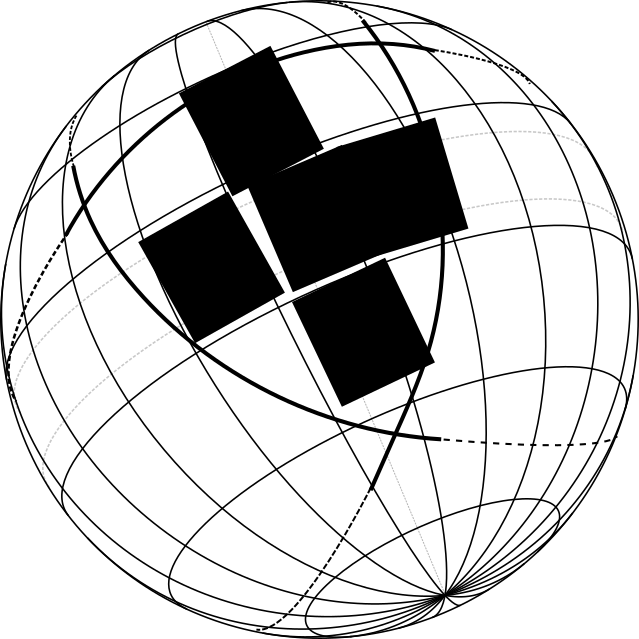
\includegraphics[width=0.5\linewidth]{./figures/title/mtvmtl.pdf}
	
	~\\[20pt]

  {\huge{Master Thesis}}\\[2.5cm]

  {\emph{written by}}\\
  {\large Pascal Debus}
  \\[0.6cm]
  {\emph{supervised by}}\\
  Markus Sprecher{\emph{,}}\\
  Prof. Dr. Philipp Grohs\\

  Seminar for Applied Mathematics\\
  ETH Zurich
  \\[0.5cm]
  {October 1, 2015}
\end{center}
\begin{tikzpicture}[remember picture,overlay]
   \node[anchor=north west,inner sep=40pt] at (current page.north west)
              {\includegraphics[scale=0.15]{./figures/title/ETHlogo.png}};
   \node[anchor=south east,inner sep=40pt] at (current page.south east)
              {\includegraphics[scale=0.25]{./figures/title/sam_logo.png}};
\end{tikzpicture}
\end{titlepage}


\providecommand{\keywords}[1]{\textbf{Key words.} #1}

\begin{abstract}
In this thesis, a versatile, multi-threaded C++ template library for 
total variation (TV) minimization of manifold-valued image data is introduced. 
The library implements two minimizers: the iteratively reweighted least squares (IRLS) algorithm using the Riemannian
Newton method for the optimization step and the proximal point algorithm.
Pixels can take values in Euclidean space, on the Sphere, the special orthogonal group, 
the set of positive definite matrices and the Grassmann manifold while images can be either two-
or three-dimensional. Some semi-analytic expressions for the derivatives of the squared
distance functions using Kronecker products and a short overview about the relevant Grassmann manifold theory is provided along with a high level documentation of the library and its design concepts.
The last part demonstrates the library's capabilities on different applications in image and video processing, 
medical imaging and computer vision. Performance is measured and compared for the IRLS and the proximal point
implementations. Lastly the influence of the noisy original data on the the minimizer is investigated.\\
\keywords{total variation minimization, manifold-valued data, iteratively reweighted least squares, proximal
point algorithm, Riemannian Newton method}
\end{abstract}


\clearemptydoublepage
\tableofcontents

\clearemptydoublepage
\phantomsection
\addcontentsline{toc}{chapter}{\listfigurename}
\listoffigures

\clearemptydoublepage
\phantomsection
\addcontentsline{toc}{chapter}{\listtablename}
\listoftables

\clearemptydoublepage
\phantomsection
\addcontentsline{toc}{chapter}{\listalgorithmname}
\listofalgorithms

%\clearemptydoublepage

\glsaddall
\cleardoublepage
\phantomsection
\addcontentsline{toc}{chapter}{List of Abbreviations}
\printnoidxglossary[type=abbrev,sort=letter,style=index]

\clearemptydoublepage

\begin{chapter}{Introduction}
\label{ch:introduction}
Various forms of noise occur in many forms of data acquisiation, transmission and processing.y
This noise needs to be removed in order to obtain a meaningful interpretation of the data, to enable further processing or, as in many image processing 
applications, just for aesthetical reasons. A common everyday example for a noisy image is taking a picture with a digital camera (e.g. integrated in a smart phone) in a weakly illuminated room:
Especially the dark areas of the picture are not uniform in color and brightness but have small variations from pixel to pixel.\\

A noise removal algorithm needs to remove these small variations but at the same time not alter important features of the data. In the case of images important features are for example 
the edges separating areas of different colors and providing the necessary sharpness of the picture. These edges on the other hand are characterized by large variations. This distinction
between small and large variations is also helpful in the task of inpainting, which tries to restore the picture at unknown or damaged regions.\\

The method of total variation(TV) noise removal, which has the above described capabilities, was first introduced by Rudin, Osher and Fatemi \cite{RudinOsher} in 1992
for the case of real-valued, that means grayscale images. Their method is briefly summarized in the following section.

\section{Grayscale images}
Let $u_0: \Omega\subset \mathbb{R}\to \mathbb{R}$ desribe the original, noise-free image, where the image domain $\Omega$ is usually a rectangular or cuboid subset of $\mathbb{R}^2$ or $\mathbb{R}^3$, respectively. 
Assuming the original pictures is corrupted by gaussian noise $n: \Omega\to\mathbb{R}$ with zero mean and variance $\sigma^2$ the noisy picture is given by $u: \Omega\to \mathbb{R}$, where
$u = u_0 + n$. The edge preserving denoising of the picture is then equivalent to the solution $u^* :\Omega\to \mathbb{R}$ of the following constrained optimization problem:
\begin{align}
    \label{osher_opt}
    u^* &= \operatorname{argmin}_{f: \Omega\to \mathbb{R}}\int_\Omega\left\vert\nabla u\right\vert  \quad\text{s.t.}\\
    \int_\Omega(u-u_0) &= 0, \quad\text{and} \int_\Omega(u-u_0)^2 = \sigma^2
\end{align}

The first term $TV(u)=\int_\Omega\left\vert\nabla u\right\vert$ is called the total variation of $u$. Rudin, Osher and Fatemi then use a partial differential equation (PDE) approach to solve
the corresponsing Euler-Lagrange equation for (\ref{osher_opt}). Later Chambolle and Lions \cite{ChambolleLions} showed that (\ref{osher_opt}) is equivalent to the minimization of
the functional
\begin{equation}
    \label{osher_func}
    \frac{1}{2}\norm{u-u_0}_2^2 +\lambda \int_\Omega\left\vert\nabla u\right\vert
\end{equation}

\subsection{Edge preservation} % (fold)
\label{sub:Edge preservation}
A basic intuition why the $L^1$ norm in (\ref{osher_func}) is besser suited for conserving sharp discontinuities such as edges can be seen from the following plot.\\

\begin{figure}[h!]
        \centering
	    \includegraphics[width=0.9\linewidth]{./figures/introduction/tv12comparison.pdf}
	\caption[Comparison total variation]{Plots of three functions with ($N=1,\;10,\;100$) steps and a total variation equal to $1.0$}
	\label{fig:tv12comparison}
\end{figure}
\begin{table}[h!]
\centering
\begin{tabular}{|l|l|l|}
    \hline
    \textbf{Function} & $\int_{[0,1]}\left\vert\nabla f\right\vert$ & $\int_{[0,1]}\left\vert\nabla f\right\vert^2$ \\
    \hline
    $f_1$ & 1.0 & 1.0 \\
    $f_2$ & 1.0 & 0.1 \\
    $f_3$ & 1.0 & 0.01 \\
    \hline
\end{tabular}
\end{table}

One can see that the $L^2$ variation term favors continuous transitions such as $f_3$ rather than the sudden jump in $f_1$ whereas the total variation is the same for
all cases.
% subsection Edge preservation (end)

\section{Color Images}
The next step in the development of image denoising algorithms was their generalization to color images. From a mathemtical perspective this just means considering pictures
from $\Omega\to C\simeq \mathbb{R}^3$ where the form and additional properties of $C$ depend on the chosen color model. \\
In the most simple case of linear models, like RGB for instance, one could choose $C$ as $[0,1]^3$ and consider denoising each component individually (channel-by-channel model)
or consider $\mathbb{R}^3$ as a normed vector space of tuples $(x_R, x_G, x_B)$ (linear-vectorial model).\\
For the nonlinear models, especially the so-called chromaticity-brightness model, Chang and Kang \cite{ChangKuang} showed the closest resemblance to human perception.
In this case we can take $C=S^2\times [0,1]$ such that the chromatictiy takes values on the sphere $S^2$ considered as a submanifold of the euclidian space $\mathbb{R}^3$, 
while the brightness is real-valued, as in the case of graysale images.

\section{Manifold-valued Images} % (fold)
\label{sec:Manifold-valued Images}
In the last section we have already seen that, depending on the chosen color model, pixels can take their values on a manifold and are usually represented by their matrices.
This data arises in a variety of application such as Diffusion Tensor Magnetic Resonance Imaging (DTI-MRI), computer vision and robotics to name just a few.

\section{Objective and Outline of this work}
In this work we will introduce an extendable multi-threaded C++ template library for the purpose of TV Minimization of manifold-valued images. 
So far the implemented minimization algorithms are based on the iteratively reweighted least squares (IRLS) adaption suggested by Sprecher and Grohs \cite{SprecherIRLS} as well as a 
proximal point algorithm by Weinmann et al \cite{WeinmannPRPT}. We extend the implementation to 3D images cubes, the Grassmann manifold and also provides some quasi-analytic expressions
for derivatives of the Riemannian distance function.\\

In the following chapter 2 a short summary of the necessary theory, a description of the algorithms and relevant properties for each of the implemented manifolds.
After that the chapter 3 introduces the library itself in particular its capabilieties, design concepts, structure, installation and usage in the form of some typical
use cases. In Chapter 4 numerical experiments are conducted, showing various application of the library as well as convergence behavior and comparisons between 
IRLS and proximal point based minimizers.\\

Finally, chapter 5 concludes with possible extensions and adaptions of the library, in particular possibility of recursive splitting of the image domain into smaller subproblems and
the transition to distributed architectures.
% section Manifold-valued Images (end)
\end{chapter}


\clearemptydoublepage

\begin{chapter}{Theory}
\label{ch:theory}

\section{Riemannian Newton Method} % (fold)
\label{sec:Riemannian Newton Method}

% section Riemannian Newton Method (end)

\section{Algorithms} % (fold)
\label{sec:Algorithms}

\subsection{IRLS} % (fold)
\label{sub:IRLS}

% subsection IRLS (end)

\subsection{Proximal Point} % (fold)
\label{sub:Proximal Point}

% subsection Proximal Point (end)

% section Algorithms (end)

\section{Manifolds} % (fold)
\label{sec:Manifolds}

\subsection{Euclidian} % (fold)
\label{sub:Euclidian}

% subsection Euclidian (end)

\subsection{Sphere $S^n$} % (fold)
\label{sub:Sphere}

% subsection Sphere (end)

\subsection{Special Orthogonal Group SO(n)} % (fold)
\label{sub:SO(N)}

\subsubsection{Second derivatives of the distance function} % (fold)
\label{ssub:Second derivatives of the distance function}
For the computation of the second derivatives we can take the expression obtained using the above theorem as a starting point and follow the approach and notation of Magnus \cite{magnus}. 
This allows us to express the derivatives as combinations of simple Kronecker product of the arguments which also is very straightforward and compact to implement. 
The detailed derivations can be found in the appendix \ref{appendix} while here we only represent the final results. \\
For the second derivative with respect to the first argument one readily arrives at
\begin{equation}
    \label{eq:son_xx_der}
    \frac{\partial^2 d^2(X,Y)}{\partial X\partial X} = -2\left[\left(\left(\log X^TY\right)^T\otimes\mathbbm{1}_n\right) + \left(\mathbbm{1}_n\otimes X \right)\operatorname{D}\log(X^TY) \left(Y^T\otimes\mathbbm{1}_n \right) K_{nn}\right],
\end{equation}
where $K_{nn}$ denotes the commutator matrix which transforms the columnwise vectorization of a matrix $A$ to the vectorization of its tranpose $A^T$.\\

The mixed derivative is given by
\begin{equation}
    \label{eq:son_xy_der}
    \frac{\partial^2 d^2(X,Y)}{\partial X\partial Y} = -2\left(\mathbbm{1}_n\otimes X \right)\operatorname{D}\log(X^TY) \left(\mathbbm{1}_n\otimes X^T \right),
\end{equation}
These expressions are quasi-analytical: Matrix logarithms, exponentials and the Frechet derivative of the logarithms need to be evaluated numerically. Details concerning the 
implementation of the latter are postponed to section \ref{seq:frechetderivatives}.

% subsubsection Second derivatives of the distance function (end)


% subsection SO(N) (end)

\subsection{Symmetric Positive Definite Matrices SPD(n)} % (fold)
\label{sub:SPD(N)}

\subsubsection{Second derivatives of the distance function} % (fold)
\label{ssub:Second derivatives of the distance function}
For the SPD matrices we proceed in the same way as for the orthogonal group and obtain
\begin{align}
    \label{eq:spd_xx_der}
    \frac{\partial^2 d^2(X,Y)}{\partial X\partial X} &= 
    2\Bigg[
	\left(X^{-\frac{1}{2}}\log\left(X^{-\frac{1}{2}}YX^{-\frac{1}{2}}\right)^T\otimes\mathbbm{1}_n\right)
	+\left(\mathbbm{1}_n\otimes X^{-\frac{1}{2}}\log\left(X^{-\frac{1}{2}}YX^{-\frac{1}{2}}\right)\right) \\
    &	+\left(X^{-\frac{1}{2}}\otimes X^{-\frac{1}{2}}\right)\operatorname{D}\log(X^{-\frac{1}{2}}YX^{-\frac{1}{2}})\left( \left(X^{-\frac{1}{2}}Y\otimes\mathbbm{1}_n\right)
	+ \left(\mathbbm{1}_n\otimes X^{-\frac{1}{2}}Y\right)\right) 
    \Bigg] \times\cdots \nonumber \\
    & \cdots\times\left(X^{-\frac{1}{2}}\otimes X^{-\frac{1}{2}}\right)\operatorname{D}(X^{\frac{1}{2}})\nonumber
\end{align}
and for the mixed derivatives
\begin{equation}
    \label{eq:spd_xy_der}
    \frac{\partial^2 d^2(X,Y)}{\partial X\partial Y} = -2\left(X^{-\frac{1}{2}}\otimes X^{-\frac{1}{2}}\right)\operatorname{D}\log\left(X^{-\frac{1}{2}}Y X^{-\frac{1}{2}}\right)\left(X^{-\frac{1}{2}}\otimes X^{-\frac{1}{2}}\right)
\end{equation}

% subsubsection Second derivatives of the distance function (end)

% subsection SPD(N) (end)

\subsection{Grassmanian Gr(n,p)} % (fold)
\label{sub:Grassmanian}
The Grassmann manifold is special among the manifolds so far considered due to the fact that it is a quotient manifold. 
As such, there are different possbilieties for choosing equivalence classes and representatives thereof from some matrix space that need to be addressed
before an implementation.\\

For positive integers $n$ and $p\leq n$ the Grassmann manifold is defined as the set of $p$-dimensional linear subspaces of $\mathbb{R}^n$. 
Since a linear subspace $\mathcal{Y}\in Gr(n,p)$ can be specified using a basis, we can arrange its basis vectors as columns of
a matrix $Y\in\mathbb{R^{n\times p}}$ such that its column space spans $\mathcal{Y}$. The rank of $Y$ must necessarily be full and equal to $p$ because of the linear independence
of its columns. Hence, elements of $Gr(n,p)$ can be represented using elements of the \emph{non-compact Stiefel manifold}
\begin{equation}
    \tilde St(n,p) := \left\lbrace Y\in\mathbb{R}^{n\times p}:\; \operatorname{rank}Y=p\right\rbrace.
\end{equation}

\subsubsection{Quotient representations} % (fold)
\label{ssub:Quotient representations}
Observing now that post-multiplication by any invertible $G\in Gl(p)$ does not change the span of $Y$, we can form the equivalence classes
\begin{equation}
    Y\,GL(p) := \left\lbrace YG: G\in Gl(p)\right\rbrace
\end{equation}
consisting of all matrices having the same span as $Y$. These equivalence classes can be thought of as the distinct elements of the Grassmannian which
leads to the following quotient manifold representation.\\
\begin{equation}
    Gr(n,p):=\tilde St(n,p) / Gl(p)
\end{equation}

This representation used by Absil et al\cite{AbsilGrasmman} which is very general because only the rank is specified. In the next steps of presenting the relavant quantities for the
algorithm we will follow Absil's derivation and notation but choose the quotient representation used by Edelman et al \cite{EAS} which is based on the orthogonal group. This will simplify the
most expressions and is also desirable from an algorithmic point of view as it removes more degrees of freedom in the choice of possbily unique representatives.\\

For the sake of completeness we also mention a completely different approach by Sato and Iwai \cite{SatoIwai} who choose $\mathbb{R}^{n\times n}$ as embedding space
where elements of $Gr(n,p)$ are given by rank $p$ orthogonal projection matrices. The presented application are, however, mostly eigenvalue problems while in the case
of image denoising the increased memory requirements are disadvantageous.\\

The orthogonal group quotient represenation of the Grassmann manifold is given by
\begin{equation}
    Gr(n,p) = St(n,p) / O(p) %= O(n) / (O(p) \times O(n-p)),
\end{equation}
where we denote by $St(n,p)=\left\lbrace Y\in\mathbb{R}^{n\times p}:\; Y^TY=\mathbbm{1}_p,\right\rbrace$ the \emph{compact} Stiefel manifold with the additional
requirement that the basis spanning the subspace $\mathcal{Y}$ be orthonormal now. The canoncial quotient projection map is then given by
\begin{equation}
    \pi : St(n,p)\ni Y \mapsto \operatorname{span} Y=\mathcal{Y} \in Gr(n, p)
\end{equation}
% subsubsection Quotient representations (end)

\subsubsection{Locally unique representatives} % (fold)
\label{ssub:Locally unique Representative}
Let $U\in St(n,p)$ and define the local affine cross section through $U$ and orthogonal to the fiber $U[O(p)]=\pi^{-1}(\mathcal{U})\subset St(n,p)$ by
\begin{equation}
    S_U := \left\lbrace V\in St(n,p): U^T(V-U)=0 \right\rbrace\subset St(n,p).
\end{equation}

The equivalence class of $V\in St(n,p)$ is equal to $\pi^{-1}(\pi(V))=V\,O(p)$ and to calculate its intersection with $S_U$ we choose $R\in O(p)$ such that
$VR\in VO(p)$ and obtain
\begin{align}
    VR\in S_U\;\Leftrightarrow\; U^T(VR-U)=0 \;\Leftrightarrow\; R = (U^TV)^{-1}
\end{align}
which leads to the intersection
\begin{align}
    S_U \cap V[O(p)] = \left\lbrace VR = V(U^{T}V)^{-1} \right\rbrace .
\end{align}
which can be also empty if $U^{T}S$ is not invertible. Finally, we define a \emph{cross-section mapping} $\sigma_U$ restricted to the set
\begin{equation}
    \mathcal{U}_U := \left\lbrace\mathcal{V}=\operatorname{span}V:\; U^TV\in GL(p) \right\rbrace
\end{equation}
by 
\begin{equation}
    \sigma_U: Gr(n,p)\supset \mathcal{U}_U\ni\mathcal{V}=\operatorname{span}V\mapsto V(U^{T}V)^{-1} \in S_U \subset St(n,p).
\end{equation}
which is a diffeomorphism providing the differentiable structure considering the embedding of $St(n,p)$ in Euclidian space.\\

The above considerations are important for the design of algorithms for two reasons.\\
Firstly, it provides the means to give well-defined expressions for various quantities we want to compute using arbitrary representatives.
For the case of an average for instance, we can take representatives $Y_1,\ldots,Y_n\in St(n,p)$ for $\mathcal{Y}_1,\ldots,\mathcal{Y}_n\in Gr(n,p)$
and find a $U\in St(n,p)$ such that $S_U$ has non-zero intersection with all the $Y_i$'s equivalence classes, which is equivalent
to $U^TY_i\in Gl(p)$. The average $\mathcal{A}$ can then be written as
\begin{equation}
    \mathcal{A} := \pi\left(\sum_{i=1}^{n}\sigma_U(Y_i)\right)=\pi\left(\sum_{i=1}^{n}Y_i(U^{T}Y_i)^{-1}\right).
\end{equation}

Secondly, it allows us to find a parametrization of $Gr(n,p)$ in terms of $\mathbb{R}^{n\times p}$ matrices. This is necessary to construct a local basis of the tangent base
and make the dimension of the sparse linear system a function of the intrinsic manifold dimension $(n-p)p$ instead of the embedding dimension $np$.
% subsubsection Locally unique Representative (end)

\subsubsection{Tangent space} % (fold)
\label{ssub:Tangent space}
Due to the quotient structure which forces us to work with representatives we cannot just use the usual method for finding the tangent space by differentiating
curves on the manifold but have to start with "numerator" of the quotient $St(n,p)$ instead. For the Grassmann manifolds only tangent vectors of a special subspace of $T_YSt(n,p)$,
the horizontal space, can modify the span of subspace and exactly those belong to the tangent space of $Gr(n,p)$. \\

Let $Y\in St(n,p)\subset\mathbb{R}^{n\times p}$. Then tangent space at $Y$ (\cite{AbsilOptim} for details of the derivation) to the compact Stiefel manifold is given by
\begin{align}
    \label{eq:stiefel_tangentspace}
   T_YSt(n,p)	&= \left\lbrace Z\in\mathbb{R}^{n\times p}: Y^TZ+Z^TY=0 \right\rbrace\\
   &=  \left\lbrace Y\Omega + Y_{\bot}K: \Omega\in\operatorname{Skew}(p),\, K\in\mathbb{R}^{(n-p)\times p} \right\rbrace\nonumber
\end{align}
where $Y_{\bot}\in\mathbb{R}^{(n\times (n-p)}$ is defined such that $[Y,Y_{\bot}]\in O(n)$. The second representation of (\ref{stiefel_tangentspace})
already implies the decomposition into vertical and horizontal spaces we are going to perform next.

The vertical space at $Y$ is by definition the tangent space to the fiber $\pi^{-1}(\pi(Y))$
\begin{equation}
    \label{eq:stiefel_horizontalspace}
    V_Y = T_Y\pi^{-1}(\pi(Y))=T_YY[O(p)]=Y[\operatorname{Skew}(p)],
\end{equation}
while the horizontal space is defined as its orthogonal complement with respect to (\ref{eq:stiefel_tangentspace})
\begin{equation}
    \label{eq:stiefel_verticalspace}
    H_Y=V_Y^{\bot} =\left\lbrace H\in T_Y St(n,p):Y^TH=0 \right\rbrace \simeq Y_{\bot}[\mathbb{R}^{(n-p)\times p}].
\end{equation}

Using this, the tangent space to $Gr(n,p)$ at $\pi(Y)=\mathcal{Y}$, along with its projector is given by 
\begin{align}
    \label{eq:grassmann_tangentspace}
    T_{\mathcal{Y}}Gr(n,p)&\simeq  H_YSt(n,p)\simeq Y_{\bot}[\mathbb{R}^{(n-p)\times p}]\\
    \pi_{Y_{\bot}}&:=\mathbbm{1}_n-YY^T
\end{align}


% subsubsection Tangent space (end)

\subsubsection{Exponential map} % (fold)
\label{ssub:Exponential map}
Let $X, Y$ span $\mathcal{X}, \mathcal{Y}$, respectively and let $U\Sigma V^{T}$ denote the compact singular value decomposition of $Y$. Then
\begin{equation}
    \operatorname{Exp}_{\mathcal{X}}(\mathcal{Y})=\operatorname{span}\left( XV\cos\Sigma + U\sin\Sigma\right).
\end{equation}
% subsubsection Exponential map (end)



\subsubsection{Distance function} % (fold)
\label{ssub:Distance function}
Using the previously defined exponential map, one can easily define a geodesic distance function on the Grassmann manifold which is induced by its Riemannian metric
\begin{equation}
    g(X,Y) = \tr X^TY
\end{equation}
Then the distance function is given by the principal angles $\theta_i$ between the subspaces 
\begin{equation}
    \label{eq:gr_geod_dist}
    d_g^2(X,Y) = \norm{\theta}_2^2=\sum_{i=1}^p\theta_i^2,
\end{equation}
where the the principal angles can be obtained by computing the singular value decomposition of $X^TY$.

\begin{align}
    X^TY &= U\Sigma V^T = U\cos\Theta V^T\\
    \Sigma &= \operatorname{diag} (\sigma_1,\cdots,\sigma_p)\\
    \Theta &= \operatorname{diag} (\theta_1,\cdots,\theta_p) = \operatorname{diag} (\arccos\sigma_1,\cdots,\arccos\sigma_p)
\end{align}

The distance function (\ref{eq:gr_geod_dist}) has the disadvantage that due to the occurence of the cosine no analytic derivatives can be computed.\\

To avoid this problem, we follow Absil's \cite{absil_GR} approach and choose an equivalent norm, the so-called projection Frobenius norm, given by

\begin{equation}
    d_P^2(X,Y) = \frac{1}{2}\norm{XX^T-YY^T}_{F}^{2} = \sum_{i=1}^p\sin^2\theta_i
\end{equation}


% subsubsection Distance function (end)


\subsubsection{First derivatives of the distance function} % (fold)
\label{ssub:First derivatives of the distance function}

\begin{equation}
    \label{eq:gr_x_der}
    \frac{\partial d^2(X,Y)}{\partial X} = 2\left(XX^T-YY^T\right)X
\end{equation}


% subsubsection First derivatives of the distance function (end)

\subsubsection{Second derivatives of the distance function} % (fold)
\label{ssub:Second derivatives of the distance function}

\begin{equation}
    \label{eq:gr_xx_der}
    \frac{\partial^2 d^2(X,Y)}{\partial X\partial X} = 2
    \left[
	\left(X^TX\otimes \mathbbm{1}_{n}\right) 
	+ \left(\mathbbm{1}_p\otimes (XX^T-YY^T)\right)
	+ \left(X^T\otimes X\right)K_{np}
    \right]
\end{equation}

The mixed derivative is given by
\begin{equation}
    \label{eq:gr_xy_der}
    \frac{\partial^2 d^2(X,Y)}{\partial X\partial Y} = -2\left[\left(X^TY\otimes \mathbbm{1}_{n}\right) + \left(X^T\otimes Y\right)K_{np}\right]
\end{equation}


% subsubsection Second derivatives of the distance function (end)


% subsection Grassmanian Gr(N,P) (end)

% section Manifolds (end)

\section{Fr\'{e}chet derivatives of matrix logarithm and square root} % (fold)
\label{sec:frechetderivatives}
To use the derivative expression computed above we need the so called Kronecker form of the Fr\'{e}chet derivative. The Fr\'{e}chet derivative
of a matrix valued function $f:\mathbb{R}^{n\times n}\to\mathbb{R}^{n\times n}$ at a point $X\in\mathbb{R}^{n\times n}$ is a linear function mapping $E\in\mathbb{R}^{n\times n}$
to $L_f(X,E)\in \mathbb{R}^{n\times n}$ such that
\begin{equation}
    f(X+E) - f(X) - L_f(X,E) = \mathcal{o}(\norm{E}).
\end{equation}
Chain rule and inverse function theorem also hold for the Fr\'{e}chet derivative:
\begin{align}
    L_{f\circ g}(X, E) &= L_{f}(g(X)),L_{g}(X,E))\\
    L_{f}(X, L_{f^{-1}}(f(X),E)) &= E
\end{align}

As we did in our formulation of the derivatives of the distance function, it can also be represented in the Kronecker form in which is represented as map
$K_f:\mathbb{R}^{n^2}\to\mathbb{R}^{n^2}$, such that $K_f(X)\in \mathbb{R}^{n^2\times n^2}$ is defined by
\begin{equation}
    \label{eq:kronckerform}
    \operatorname{vec}(L_f(X,E))=K_f(X)\operatorname{vec}(E)
\end{equation}
where $\operatorname{vec}:\mathbb{R}^{n\times n}\to\mathbb{R}^{n^2}$ denotes the columnwise vectorization operator.

\subsection{Derivative of the matrix square root} % (fold)
\label{sub:Derivative of the matrix square root}
We start by considering the Fr\'{e}chet derivative of $f(X)=X^2$, which is given by
\begin{equation}
    L_{X^2}(X,E) = XE + EX.
\end{equation}
Applying the inverse function theorem consequently leads to
\begin{equation}
    L_{X^2}(X^{\frac{1}{2}},L_{X^{\frac{1}{2}}}(X,E))=X^{\frac{1}{2}}L_{X^{\frac{1}{2}}}(X,E) + L_{X^{\frac{1}{2}}}(X,E)X^{\frac{1}{2}} = E,
\end{equation}
where the last equality shows that the Fr\'{e}chet derivative of the matrix square root $L_{X^{\frac{1}{2}}}(X,E)$ satisfies the Sylvester equation 
\begin{equation}
    \label{eq:sylvester}
    X^{\frac{1}{2}}L + LX^{\frac{1}{2}} = E,\quad L:=L_{X^{\frac{1}{2}}}(X,E).
\end{equation}

The Kronecker representation $K_{X^{\frac{1}{2}}}$ can now be obtained be using the vectorization operator on both sides of the equation and rearrange the term
to the form (\ref{eq:kronckerform}) which leads to
\begin{equation}
    K_{X^{\frac{1}{2}}}(X)=\left[\left(\mathbbm{1}\otimes X^{\frac{1}{2}}\right)+\left(X^{\frac{1}{2}T}\otimes \mathbbm{1}\right) \right]^{-1}.
\end{equation}
However, this straightforward approach has the disadvantage that the inverse of a $n^2\times n^2$ matrix need to be computed which has complexity
$\mathcal{O}((n^2)^3)=\mathcal{O}(n^6)$. In addition to that, the inverse needs to be found explicitly which is not numerically stable in general.\\

The Sylvester equation (\ref{eq:sylvester}), on the other hand, can be solved with $\mathcal{O}(n^3)$ operations via Schur transformation. We choose $E^{ij}$, the single-entry
matrices having 1 at $(i,j)$ and zero everywhere else, as a basis for $\mathbb{R}^{n\times n}$ and solve the Sylvester equation for each of the $n^2$ 
basis matrix elements. By that, the total complexity can be reduced to $n^2\mathcal{O}(n^3)=\mathcal{O}(n^5)$ and we avoid the 
potentially problematic explicit computation of inverses altogether.\\

We then obtain the final Kronecker form of the derivative by constructing its rows from the vectorized, tranposed Fr\'{e}chet derivatives:
\begin{equation}
    \left(K_{X^{\frac{1}{2}}}\right)_{in + j,\cdot} = \operatorname{vec}\left(L_{X^{\frac{1}{2}}}(X,E^{ij})^T\right) 
\end{equation}

\subsection{Derivative of the matrix logarithm} % (fold)
\label{sub:Derivative of the matrix logarithm}
For the logarithm we follow the approach described by Al-Mohy et al \cite{almohy_frechetlog} which is based on the differentiation of the Pad\'{e} approximant to $\log(1+X)$.
Since this is only applicable if the norm of $X$ is sufficiently small, the  use of an inverse scaling and squaring technique based on the relation
\begin{equation}
    \log(X) = 2\log(X^{\frac{1}{2}})
\end{equation}
is necessary.\\

Application of the chain rule leads to
\begin{equation}
    L_{\log}(X,E_0) = 2\log\left(X^{\frac{1}{2}},L_{X^{\frac{1}{2}}}(X,E_0)\right).
\end{equation}
The second argument on the right hand side can again be written as solution $E_1:=L_{X^{\frac{1}{2}}}(A,E_0)$ of an Sylvester-type equation
\begin{equation}
    X^{\frac{1}{2}}E_1+E_{1}X^{\frac{1}{2}}=E_0.
\end{equation}
Repeating the procedure $s$ times results in
\begin{align}
    L_{\log}(X,E_0)&=2^sL_{\log}\left(X^{\frac{1}{2^s}},E_s\right)\\
    X^{\frac{1}{2^{i}}}E_i+E_iX^{\frac{1}{2^{i}}}&=E_{i-1},\quad i=1,\ldots,s
\end{align}
where $E_s$ is obtained by successivly solving the set of Sylvester equations defined in the second line.\\

Finally, the Pad\'{e} approximant of order $m$ in its partial fraction form \cite{highham_pade} is given by
\begin{equation}
    \label{eq:pade_log}
    r_m(X) = \sum_{j=1}^{m}\alpha_j^{(m)}(\mathbbm{1}+\beta_j^{(m)}X)^{-1}X
\end{equation}
where $\alpha_{j}^{(m)},\beta_{j}^{(m)}\in (0,1)$ are the $m$-point Gauss-Legendre quadrature weights and nodes.\\

The derivative of (\ref{eq:pade_log}) is then easily computed as 
\begin{equation}
    L_{r_m}(X,E) = \sum_{j=1}^m\alpha_j^{(m)}(\mathbbm{1}+\beta_j^{(m)}X)^{-1}E(\mathbbm{1}+\beta_j^{(m)}X)^{-1}
\end{equation}
which leads to the final approximation of the matrix logarithm derivative, 
\begin{equation}
    \label{eq:dlog_approx}
    L_{\log}(X,E)\approx 2^{s}L_{r_m}\left(X^{\frac{1}{2^s}}-\mathbbm{1},E_s \right).
\end{equation}

For the implementation of (\ref{eq:dlog_approx}) we use algorithm 5.1 from \cite{almohy_frechetlog} with fixed $m=7$.
The Kronecker representation is then constructed as in the square root case.
% subsection Derivative of the matrix logarithm (end)




% subsection Derivative of the matrix square root (end)


% section Frechet derivative of the matrix logarithm and square root (end)


\end{chapter}


\clearemptydoublepage

\begin{chapter}{The Manifold Total Variation Minimization Template Library}
\label{ch:library}

The manifold total variation minimization template library (MTVMTL), which was developed in the course of this thesis is an easy-to-use, fast C++14 template library for TV minimization of manifold-valued two- or three-dimensional images. \\

The following chapter summarizes the capabilities of the library
and introduces into its architecture from a software engineering as well as high performance computing point of view. The last part,
describing the components in more detail, can also be understood as a high level documentation of the library and includes some basic tutorial on its usage.


\section{Capabilities} % (fold)
\label{sec:Capabilities}
The following list provides a first overview of the implemented features. More detailed
information are found in the description of the components in Section \ref{sec:Components}
and the examples in Section \ref{sub:tutorial}.
\subsection*{Manifolds} % (fold)
\label{sub:supportedManifolds}
\begin{itemize}
    \item Real Euclidean space $\mathbb{R}^n$
    \item Sphere $S^n=\left\lbrace x\in\mathbb{R}^{n+1}:\; \norm{x}=1\right\rbrace$
    \item Special orthogonal group $SO(n)=\left\lbrace Q\in\mathbb{R}^{n\times n}:\; QQ^T=\mathbbm{1}, \operatorname{det}(Q)=1 \right\rbrace$
    \item Symmetric positive definite matrices $SPD(n)=\left\lbrace S\in\mathbb{R}^{n\times n}:\; S=S^T, x^TSx>0\; \forall x\in\mathbb{R}^n\setminus\lbrace 0\rbrace \right\rbrace$
    \item Grassmann manifold $Gr(n,p) = St(n,p) / O(p)$
\end{itemize}
% subsection Supported Manifolds (end)

\subsection*{Data} % (fold)
\label{sub:Data}
\begin{itemize}
	\item 2D and 3D images
	\item Input/Output via OpenCV integration supporting all common 2D image formats
	\item CSV input for matrix valued data
	\item Input methods for raw volume image data as well as the NIfTI \cite{nifti} format for DT-MRI images
	\item Various methods to identify damaged areas for inpainting
\end{itemize}
% subsection Data (end)

\subsection*{Functionals} % (fold)
\label{sub:Functionals}
\begin{itemize}
    \item isotropic (only possible for IRLS) or anisotropic TV functionals
    \item first order TV term
    \item weighting and inpainting possible
\end{itemize}
% subsection Functionals (end)

\subsection*{Minimizer} % (fold)
\label{sub:Minimizer}
\begin{itemize}
	\item Iteratively reweighted least squares using Riemannian Newton method
	\item Proximal point
\end{itemize}
% subsection Minimizer (end)

\subsection*{Visualizations} % (fold)
\label{sub:Visualizations}
\begin{itemize}
    \item OpenGL rotated cubes visualization for SO(3) images
    \item OpenGL ellipsoid visualization for SPD(3) images
    \item OpenGL volume renderer for 3D volume images
\end{itemize}
% subsection Visualization (end)

% section Capabilities (end)

\section{Design concepts} % (fold)
\label{sec:Design}
The next sections give more insights in the implementation details of the algorithms introduced in the last chapter.
The first part discusses the performance relevant changes in data representation and computation
with respect to the Matlab prototype, which is followed by a discussion of structural changes to make
MTVMTL as modular and extendable as possible.\\

The next part is then dedicated especially to the question where and how parallelization is used in the implementation.
A related question is also the use of new language features of the C++11 and C++14 language standards 
which allow for a real compact formulation of the parallel code segments. 
The section closes with a short description of those features.

\subsection{Goals} % (fold)
\label{sub:Goals}
Traditionally, there has always been a trade-off between performance and usability requirements such as
maintainability or extendability. A good example for that is the Basic Linear Algebra Subprograms 
(BLAS) library, written in Fortran, and still considered one of the fastest libraries in existence. 
For supercomputers, even versions with hand-optimized assembly code are used, nevertheless calling
the library directly from another high level language like C or C++ is quite cumbersome. The code becomes
larger and much harder to read. \\

Languages like C++, on the other hand, offer a lot of expressive power and make it possible, through object oriented
generic programming, to write compact, reusable and even fast, though not as fast as Fortran, code. Nevertheless,
with the development of template metaprogramming techniques C++ is able to avoid the performance-usability
trade-off to a certain degree, using very elaborate compile time optimizations. Classical examples for these techniques are expression templates \cite{blitz}, also used by the Eigen linear algebra library, and specifically variadic templates, as used by MTVMTL.
C++ was consequently the ideal choice for achieving high performance and the usability requirements.

\subsubsection{Performance} % (fold)
\label{ssub:Performance}
Since the core parts of the implementation are originally based on a Matlab prototype by Sprecher \cite{SprecherIRLS}, \cite{manuel} and \cite{mara}, one of the most important
goals was a faster implementation with a smaller memory footprint. On the test platform with two hyper-threaded 2.8GHz cores (Intel i5-2520) with AVX vector extensions,
the Matlab implementation froze for images larger than one Megapixel(MP).\\

Hence, the C++ implementation should enable the algorithm to be tested in a much broader scope which is
also closer to common picture sizes in image processing, especially since even smart phones today easily produce pictures in the Megapixel range.
In addition to that, also other factors affecting the performance of the algorithm, such as cache locality and memory speed, can be investigated.\\

The main performance driver for this library is the multilevel-parallelization. Evidently, this does not include the formulation of the IRLS minimization algorithm itself, due to the fact that
it is naturally an iterative method, but rather any possible subtask such as computation of the functional values, gradient and Hessian, for example. On top of that, it was tried to
maximize cache locality on the loop level and free memory as soon as possible.
On the other hand, data that is used very often and requires costly recomputation, like the IRLS weights, are kept in memory.\\ 

In contrast to the original Matlab implementation, the computation of various quantities such as weights, first and second derivatives is not realized with tensor products any more.
For Matlab, due to the low speed of its internal loop constructs, the approach is justified but in a pure C++ implementation other factors are more important.
One reason for the change is improved readability and maintainability of the code, since tensor products usually tend to become very convoluted,
especially for the manifolds with matrix representations. Also the modularization of the manifold class is not straightforward any more, because the tensor products cannot be expressed as binary operation depending on two manifold data points.\\

From a performance and parallelization perspective, contractions of tensor products are similar to matrix products and usually require some sort of blocking scheme for parallelization.
In addition to that, because certain reshapes of the image container prior to the computation are necessary, the dimensions to be summed over are not necessarily contiguous in memory.
A high cache utilization is consequently more difficult to achieve.\\
Finally, in order to formulate certain operations as tensor products, temporary tensors of the correct dimensionality need to be created, which increases the memory consumption.\\

Another measure that significantly reduces the memory footprint for the IRLS minimizer, especially for manifolds with matrix representations, is to only save gradient and Hessian
in their local tangent space basis representation, such that the degrees of freedom correspond the intrinsic manifold dimension and not the dimension of the embedding space. This also reduces
the time to solve the sparse linear system.\\
% subsubsection Performance (end)

\subsubsection{Modularization and Extendability} % (fold)
\label{ssub:Modularization}
In principle the programming paradigm in Matlab is still procedural resulting in a hierarchy of functions for the various tasks. Handling different types of manifolds
then usually requires \texttt{switch} expressions in all functions that use manifold-specific functionality. Adding support for a new manifold to the algorithm or modifying
existing manifold functionality makes a modification of all \texttt{switch} cases necessary. There is no single point of change but many source files need to be edited.\\

For the MTVMT Library an object oriented and generic programming approach was chosen, which tries to model each variable component of the algorithm in a separate class, as 
independent of the other components as possible. For general information on C++ design paradigm see, for example, \cite{CPPTemplateMP} or \cite{CPPGeneric}.
Differences in each class are represented by specializations of their primary class template. The best example for that is the
manifold class which has a specialization for every supported manifold type and due to the fact that the functions implemented in those class specializations are generally
just functions of one or two elements of the manifold, they could also be used in other projects which require the same functionality.\\

Interfaces between classes are provided by giving classes higher in the hierarchy template parameters corresponding to lower classes: The class modelling the functional, for instance,
has a manifold type template parameter, as described in more detail in Section \ref{sec:Components}. Like all other component classes, also the functional class can be extended
by adding further specializations for other types of functionals, that include for example higher order terms or have different fidelity terms \cite{SceneFlow}.\\

Those specializations also have the advantage that the code is just in one file - a single point of change - to increase readability and maintainability.
% subsubsection Modularization (end)

% subsection Goals (end)

\subsection{Levels of parallelization} % (fold)
\label{sub:Levels of parallelization}
Parallelization takes place on two levels. The first one is shared memory multi-threading implemented with the OpenMP (OMP) language extensions. In most cases this is realized 
using the so-called \textit{pixel-wise kernels} of the Video++ (VPP) library, which makes it possible to map an arbitrary function on all pixels of a set of image containers: The function is
called for each tuple of pixels having the same coordinates in their respective image. For the parallel execution each processor is assigned a batch of image rows.
If the pixel-wise kernels are not applicable, for example if the needed subdomain of the image is too complicated, manual OpenMP loop parallelization is used. Due to the fact that the 3D pixel-wise constructs are not 
implemented in the current version of VPP, also an own 3D version of the pixel-wise kernels 
was implemented using OpenMP and variadic templates to keep the code compact.\\

The alternative to the tensor product implementation is to use pixel-wise kernels to parallelize any operation that requires iteration over an image container.
For most computations, take for instance the case of computing derivatives, only the pixel and its next neighbor in a given dimension are needed. For calculating the forward derivatives one just has to call the pixel-wise kernel with two subimages of the current working image: One with the last slice (of the given dimension) missing and one with the first slice missing. At this point it must be noted that the concept of subimages does not
involve any copies but just works by using different addressing schemes for the same
data in the memory.
The pixel-wise constructs are demonstrated in the following short Listing \ref{code:pixelwise_demo} and further illustrated in Figure\ref{fig:pixelwise_kernel}:\\

\cppinline
\begin{lstlisting}[label=code:pixelwise_demo,caption={Pixel-wise forward derivative computation}]
auto calc_first_arg_deriv = [&] (value_type& x, const weights_type& w, const value_type& i, const value_type& n) { MANIFOLD::deriv1x_dist_squared(i, n, x); x *= w; }; 

img_type YD1 = img_type(without_last_row);
vpp::pixel_wise(YD1, weightsY_ | without_last_row, data_.img_ | without_last_row, data_.img_ | without_first_row) | calc_first_arg_deriv;
\end{lstlisting}

\begin{figure}[h!]
        \centering
	    \includegraphics[width=1.0\linewidth]{./figures/library/pixelwise_kernel.pdf}
	\caption[Calculation using pixel-wise kernels]{Parallel calculation of derivatives in $y$-direction and weighting using pixel-wise kernels.
	    For each pixel position $(i,j)$ in the three input pictures, \circnum{1}, \circnum{2} and \circnum{3}, as well as in the output picture
	    \circnum{R}, the pixel-wise kernel creates a tuple $(R_{ij}, 2_{ij}, 1_{ij}, 3_{ij})=(\text{YD1}_{i,j},\text{weightY}_{i,j},\text{Image}_{i,j},\text{Image}_{i+1,j})$
	    which is than used to call the specified lambda function. Depending on the row number of the pixel, the calls are executed by different CPU cores.
	}
	\label{fig:pixelwise_kernel}
\end{figure}

The advantage is that even though some function is evaluated for a pair of neighboring pixels which are not adjacent in memory, the parallel processing is still
always row-wise. Since rows in row-major languages like C++ are contiguous in memory, one can avoid frequent memory access on distant locations and consequently avoid cache thrashing to a certain degree.\\

The second level of parallelization is instruction level parallelism, also known as \textit{Single Instruction Multiple Data} (SIMD), which uses the
processor's vector extensions (e.g. SSE, AVX, NEON).
The CPU provides some additional, special SIMD registers with increased size of usually 128 bits to 512 bits such that multiple integer or floating point variables fit inside.
Then an arithmetic operation is simultaneously applied to all variables in the register (see Figure \ref{fig:simd}) such that theoretically the amount of floating point operations is multiplied by the number
of variables fitting in the register. \\

\begin{figure}[h!]
        \centering
	    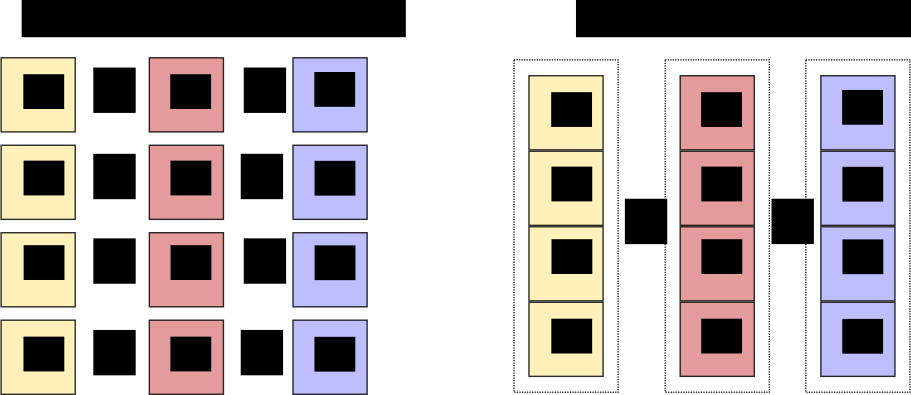
\includegraphics[width=0.7\linewidth]{./figures/library/SIMD.pdf}
	\caption[SIMD parallelization]{Instruction level parallelism using SIMD registers.
	}
	\label{fig:simd}
\end{figure}

In order to achieve this speedup the data must be aligned in memory, which means the addresses of pixels in memory must always be a multiple of the SIMD register size. Fortunately,
that issue is handled by the VPP and Eigen libraries enabling the compiler to perform the necessary vectorization optimizations.

% subsection Levels of parallelization (end)


\subsection{C++ techniques} % (fold)
\label{sub:C++ techniques}
The MTVMT Library tries to take advantage of new C++11 and C++14 language features in order to speed up computations via compile-time optimizations and also make the code
more compact and readable. The most important tools in that regard are lambda functions and variadic templates which are shortly described in the following section.
For more details check, for example \cite{CPPEleven}.

\subsubsection{Lambda functions} % (fold)
\label{ssub:Lambda functions}
A lambda function is basically a locally defined function object, which is able to capture variables from the surrounding scope. The function can but needs not to be named.
The corresponding Matlab language construct is an anonymous function or function handle, usually defined using the @ operator. The following listing
shows the basic definitions and use cases of lambda functions:\\

\cppinline
\begin{lstlisting}[label=code:lambdafun,caption={Lambda functions}]
int init = 5;
std::vector<int> v {1, 2, 3, 4};

// C++11 lambda function for adding integers
// init is captured by reference
auto f = [&] (int a, int b) {return a + b + init;};

// C++14 generic argument lambda function
// init is captured by value
auto g = [=] (auto a, auto b) {return a + b + init;};

//Call named lambda functions
int d = f(8, 3);
double e = g(1.0f, 5);

// or directly pass anonymous lambda function as argument
std::transform(v.begin(), v.end(), v.begin(), [] (auto x) { ++x; });
\end{lstlisting}

In the MTVMT library, lambda functions provide the connection between the static manifold methods and the pixel-wise kernels which apply them to the image containers.
A typical case can be seen in the already introduced listing \ref{code:pixelwise_demo}. Since lambda functions are only locally defined, in the scope where they are actually needed,
one can avoid making the method list of the classes unnecessary long.
% subsubsection Lambda functions (end)

\subsubsection{Variadic templates} % (fold)
\label{ssub:Variadic templates}
With variadic templates it is possible to define functions which take a variable number of arguments. Obviously, this is also possible in other languages like Matlab or
C with the most prominent example being the function \texttt{printf}. However, this is usually implemented using some list type (in C: \texttt{va\_list}), which adds additional 
overhead, whereas in C++ it is realized via a special kind of template metaprogramming technique, which is recursive in nature. The recursion, in turn, is resolved at compile-time
and leads to code that is actually equivalent to manually defining a function with the desired number of arguments, and consequently there is no additional runtime effort.\\

\cppinline
\begin{lstlisting}[label=code:variadic,caption={Variadic template example}]
// Recursion base case
template<typename T>
T sum(T v) {
    return v;
}

// Recursive template
template<typename T, typename... Args>
T sum(T first, Args... args) {
    return first + sum(args...);
}
\end{lstlisting}

The main application for this constructs in MTVMTL is the implementation of the Karcher mean, needed for the proximal point implementation, and MTVMTL's own version
of the 3D pixel-wise kernels.

% subsubsection Variadic templates (end)
% subsection C++ techniques (end)
% section Design (end)

\section{Components} % (fold)
\label{sec:Components}
In the following section the different components of the library are discussed. For the manifold class, this will be done in more detail to enable users to use new or customized manifold classes. A general overview of all the components is provided in Figure \ref{fig:components}.
\begin{figure}[h!]
        \centering
	    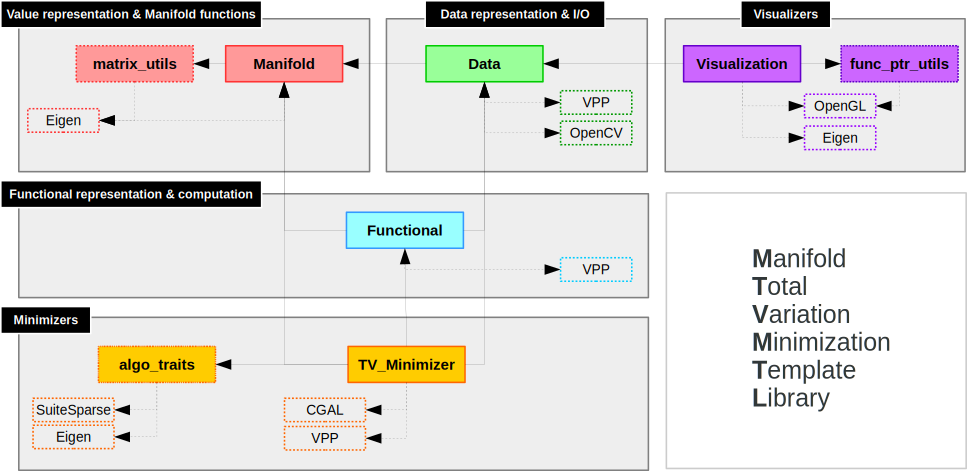
\includegraphics[width=1.0\linewidth]{./figures/library/components.pdf}
	\caption[Overview of library components]{Overview of the class hierarchy and dependencies between the library components and also third party libraries
	}
	\label{fig:components}
\end{figure}

\subsection{Manifold class} % (fold)
\label{sub:Manifold classes}
The manifold template class encapsulates all information and methods related to the differential geometric structure of the data. 
This enables the generic implementation of the functionality higher in the class hierarchy such as functional evaluations or minimizers.
The primary template has the following parameters
\cppinline
\begin{lstlisting}
// Primary Template
template <enum MANIFOLD_TYPE MF, int N, int P=0>
struct Manifold {
}; 
\end{lstlisting}
where \texttt{MF} is an enumeration constant to specify the type of the manifold, $N$ denotes the dimension of the representation space and $P$ the dimension of subspaces,
as in the case of Grassmann manifolds. In order to add a new manifold one just has to implement a specialization of this primary template.\\

So far, the manifold class contains functionality necessary for TV minimization using either the IRLS or proximal point algorithm and furthermore some additional operations
that are needed for supporting tasks like interpolation and smoothing. The class specializations are implemented using only static constants and methods: At no time it is necessary or 
desired to actually instantiate the class. The methods itself are usually unary or binary functions, with parameters and result all passed by reference to avoid copies.
Since these methods are called very often, basically for every pair of neighboring pixels, they are all declared \texttt{inline} in order to support the compiler during 
the code optimization.\\

It is also possible to use these class specializations in other projects requiring similar functionality, like 
for instance when implementing a geodesic finite element solver.\\

In the following, excerpts of the SPD implementation are shown to illustrate which information and functionality a new manifold class needs to provide and to give an overview
of the available functions.

\subsubsection{Static constants} % (fold)
\label{ssub:Static constants}
\cppinline
\begin{lstlisting}
static const MANIFOLD_TYPE MyType;	// SPD
static const int manifold_dim ;		// N*(N+1)/2
static const int value_dim;		// N*N

static const bool non_isometric_embedding;
\end{lstlisting}
The first constant just stores the manifold template parameter introduced above, while \texttt{manifold\_dim} and \texttt{value\_dim} are the intrinsic dimensions of the manifold
and of its embedding space, respectively. Finally, the Boolean constant is just a flag which tells the algorithm that special pre- and post-processing for interpolation is necessary.\\
% subsubsection Static constants (end)

\subsubsection{Type definitions} % (fold)
\label{ssub:Type definitions}
To allow the generic formulation of the algorithms, the manifold class provides a mapping between the types of their values, derivatives, tangent bases and underlying scalar type and their 
actual representation as matrix and vector data types of the Eigen linear algebra library. Examples can be seen in the following listing:

\cppinline
\begin{lstlisting}
// Scalar and value typedefs
typedef double scalar_type;
typedef double dist_type;
typedef Eigen::Matrix<scalar_type, N, N> value_type;
// ...

// Tangent space typedefs
typedef Eigen::Matrix <scalar_type, N*N, N*(N+1)/2> tm_base_type;
// ...

// Derivative Typedefs
typedef value_type deriv1_type;
typedef Eigen::sMatrix<scalar_type, N*N, N*N> deriv2_type;
typedef Eigen::Matrix<scalar_type, N*(N+1)/2, N*(N+1)/2> restricted_deriv2_type;
// ...
\end{lstlisting}
% subsubsection Type definitions (end)

\subsubsection{Static methods} % (fold)
\label{ssub:Static methods}
Finally, the following methods are implemented for the manifold classes.

\begin{description}
    
    \item[Riemannian distance function and its derivatives] \hfill \\
	\cppinline
	\begin{lstlisting}
inline static dist_type dist_squared(cref_type x, cref_type y);
// First derivatives	    
inline static void deriv1x_dist_squared(cref_type x, cref_type y, deriv1_ref_type result);
inline static void deriv1y_dist_squared(cref_type x, cref_type y, deriv1_ref_type result);
// Second derivatives
inline static void deriv2xx_dist_squared(cref_type x, cref_type y, deriv2_ref_type result);
inline static void deriv2xy_dist_squared(cref_type x, cref_type y, deriv2_ref_type result);
inline static void deriv2yy_dist_squared(cref_type x, cref_type y, deriv2_ref_type result);
	\end{lstlisting}
    
    \item[Exponential and Logarithm map] \hfill \\
	\cppinline
	\begin{lstlisting}
template <typename DerivedX, typename DerivedY>
inline static void exp(const Eigen::MatrixBase<DerivedX>& x, const Eigen::MatrixBase<DerivedY>& y, Eigen::MatrixBase<DerivedX>& result);
inline static void log(cref_type x, cref_type y, ref_type result);

inline static void convex_combination(cref_type x, cref_type y, double t, ref_type result);
	\end{lstlisting}

	The parameters of the exponential here are not the manifolds own typedefs but the base class of all Eigen matrix data types. The reason for using this construction is that the function
	can also be called with composite expressions (e.g. $XY+Z$) without a temporary copy. Most of the other functions are usually called with atomic expressions only, hence there is no
	need to use this more complicated construction on a general basis.\\
	The \texttt{convex\_combinations} method computes the point $z$ on the manifold reached by following a unit speed geodesic connecting the points $x$ and $y$ for a time $t$.

    \item[Karcher mean] \hfill \\
	\cppinline
	\begin{lstlisting}
inline static void karcher_mean(ref_type x, const value_list& v, double tol=1e-10, int maxit=15);
inline static void weighted_karcher_mean(ref_type x, const weight_list& w, const value_list& v, double tol=1e-10, int maxit=15);

// Variadic templated version
template <typename V, class... Args>
inline static void karcher_mean(V& x, const Args&... args);
	\end{lstlisting}
	
	Implementations for finding the Karcher mean of an arbitrary number of points. The first version requires the points to be stored in a \texttt{std::vector} container while
	the second version is based on variadic templates and expects the arguments just as a comma separated list after the first argument, where the final result will be stored.
	Creating the list for the first version eventually requires copying and is consequently slower but has an overloaded version which allows to compute a weighted Karcher mean
    
    \item[Tangent plane basis, projector and interpolation] \hfill \\
	\cppinline
	\begin{lstlisting}
// Basis transformation for restriction to tangent space
inline static void tangent_plane_base(cref_type x, tm_base_ref_type result);
// Projection
inline static void projector(ref_type x);
// Interpolation pre- and postprocessing
inline static void interpolation_preprocessing(ref_type x);
inline static void interpolation_postprocessing(ref_type x);
	\end{lstlisting}

	The first function computes a basis of the tangent space at the point $x$ and stores it in \texttt{result}, as columns of a matrix.\\
	The projector, if defined for the given manifold, will project a point of the ambient embedding spacing onto the manifold. This might either be an actual projector in the mathematical sense or, as in the Euclidean case, a cutoff
	function which maps the data back into the desired value range ($[0,1]^n$ in the Euclidean case). \\
	Interpolation pre- and postprocessing is necessary for instance for the SPD manifold. Other manifolds must just provide an empty implementation.
\end{description}
% subsubsection Static end)
% subsection Manifold classes(end
\subsection{Data class} % (fold)
\label{sub:Data class}
The data class handles anything related to storage, input and output of two- or three-dimensional image data, as well as some support functions for detecting edges and damaged areas in a picture.
In contrast to the manifold class, the data class needs to be instantiated such that a reference to the data object can be passed to any class which needs data access. In addition
to the dimension of the picture, the data class takes a fully specialized manifold class type as a template parameter:

\cppinline
\begin{lstlisting}
// Primary Template
template <typename MANIFOLD, int DIM >
class Data {
};    
\end{lstlisting}

There are basically four multi-dimensional arrays stored in the data class: The original noisy image, the current working image and, if applicable, arrays storing the inpainting
and edge weight information. For storage, the n-dimensional VPP \cite{VPP} image container is used.\\

This image container class works very well together with the Eigen vector and matrix data types, provides a variety of expressive loop- and iterator constructs and also takes care
of the alignment of the image data in memory, which is a prerequisite for the \textit{Single Instruction Multiple Data} (SIMD) optimization and vectorization by the compiler.
Since the memory management of the container is based on \texttt{std::shared\_pointer}, it is also very easy to efficiently access subimages or slices of an image without any copies.\\

The most common input methods for 2D and 3D are summarized in the following code snippet:
\cppinline
\begin{lstlisting}
 // 2D Input functions
void rgb_imread(std::string filename);	// for R^3
void rgb_readBrightness(std::string filename); // for R
void rgb_readChromaticity(std::string filename); // for S^2
void readMatrixDataFromCSV(std::string filename, const int nx, const int ny);

// Synthetic SO/SPD picture 
void create_nonsmooth_son(const int ny, const int nx);
void create_nonsmooth_spd(const int ny, const int nx);
 
//3D Input functions
void rgb_slice_reader(std::string filename, int num_slides); 
void readMatrixDataFromCSV(std::string filename, const int nz, const int ny, const int nx);
void readRawVolumeData(std::string filename, const int nz, const int ny, const int nx);

// OutputFunctions
void rgb_saveimage(std::string fname); // save image
void rgb_show();						//open images viewer
	
void output_matval_img(std::string filename) const; // save in CSV format
\end{lstlisting}
The purpose and usage of most of these methods is self-explanatory. The CSV readers expect the data to be a linear list of pixels, where the components of each pixel are
comma-separated and row-wise flattened, such that each line of the input file contains exactly one pixel. The order of the list is row-wise for 2D or slice-wise, then row-wise for 3D images,
respectively. \\ 
The slice reader reads a series of images, following the filename scheme \texttt{filenameX.ext}, where \texttt{X} is the number of the slice to be read into an image cube at $z$-coordinate
\texttt{X}.
% subsection Data class (end)

\subsection{Functional class} % (fold)
\label{sub:Functional class}
In addition to fully specialized Manifold and Data class types (third and fourth template parameters),
there are three further template parameters that must be specified by the library user. The first one
is the order of the functional which refers to the order of the highest differential operator in the TV term of the functional.
So far, only first order functionals are implemented which corresponds to setting \texttt{ord=FIRSTORDER} in the primary template shown below.

\cppinline
\begin{lstlisting}
//Primary Template
template <enum FUNCTIONAL_ORDER ord, enum FUNCTIONAL_DISC disc, class MANIFOLD, class DATA, int DIM=2>
class Functional{
};
\end{lstlisting}

The second template parameter \texttt{disc} determines whether the isotropic or the anisotropic version is to be used. Please note that for the proximal point algorithm only
anisotropic is available. Finally, the last parameter specifies the dimensionality of the data. \\
The main purpose of the functional class is to provide methods for the computation of all functional-related quantities, such as evaluation of the functional, its gradient,
Hessian and construction of a local basis of the tangent spaces. That also means that in the IRLS case the functional class stores the sparse linear system that needs to be solved
in each Newton step.\\

For users of the library, the most important methods are those for setting the $\lambda$ and $\epsilon^2$ parameters.
\cppinline
\begin{lstlisting}
inline param_type getlambda() const { return lambda_; }
inline void setlambda(param_type lam) { lambda_=lam; }
inline param_type geteps2() const { return eps2_; }
inline void seteps2(param_type eps) { eps2_=eps; }
\end{lstlisting}

Should it be necessary, it is also possible to access some of the stored quantities directly using
\cppinline
\begin{lstlisting}
// Evaluation functions
result_type evaluateJ();
void  evaluateDJ();
void  evaluateHJ();
 
void updateTMBase();

inline const gradient_type& getDJ() const { return DJ_; }
inline const sparse_hessian_type& getHJ() const { return HJ_; }
inline const tm_base_mat_type& getT() const { return T_; }
\end{lstlisting}
The functions in lines 3, 4 and 6 merely trigger a recomputation while the last three functions return references to these quantities. \texttt{evaluateJ()} returns the functional value and triggers the 
recomputation of the weights.


% subsection Functional class (end)

\subsection{TV minimizer class} % (fold)
\label{sub:TVMinimizer class}
For the TV minimizer class it makes sense to consider the IRLS and proximal point implementation separately. The primary template is shown in the following code snippet.
\cppinline
\begin{lstlisting}
//Primary Template 
template <enum ALGORITHM AL, class FUNCTIONAL, class MANIFOLD, class DATA, enum PARALLEL PAR=OMP, int DIM=2>
class TV_Minimizer{ 
};
\end{lstlisting}
As in the previous cases one has to provide fully specialized manifold, data and also functional types. Again, the last parameter specifies the dimension of the data. Of the
remaining two parameters, \texttt{PAR} has the default value OMP, which specifies the method of parallelization, in this case the OpenMP language extensions. Other methods, including just serial
execution, could be added later. The remaining template parameter, \texttt{AL} specifies the minimizer to be used and can take the values \texttt{IRLS} or \texttt{PRPT} (Proximal point).\\

For IRLS, the public class interface looks like\\
\cppinline
\begin{lstlisting}
void first_guess();		    // First guess for inpainting
void smoothening(int smooth_steps); // Simple averaging box filter
newton_error_type newton_step();    // perform one newton step
void minimize();		    // full minimization

// Getters and Setters for parameters
void setMax_runtime(int t) { max_runtime_ = t; }
void setMax_irls_steps(int n) { max_irls_steps_ = n; }
void setMax_newton_steps(int n) { max_newton_steps_ = n; }
void setTolerance(double t) {tolerance_ =t; }
	    
int max_runtime(int t) const { return max_runtime_; }
int max_irls_steps(int n) const { return max_irls_steps_; }
int max_newton_steps(int n) const { return max_newton_steps_; }
int tolerance(double t) const { return tolerance_; }
\end{lstlisting}

and for proximal point it is\\
\cppinline
\begin{lstlisting}
use_approximate_mean(bool u) { use_approximate_mean_ = u; } // turn mean approximation on/off
void first_guess();					    // First guess for inpainting
 
void updateFidelity(double muk);			    // Update Fidelity part
void updateTV(double muk, int dim, const weights_mat& W);   // Update TV part

void geod_mean();	    // Calculate geodesic mean
void approx_mean();	    // approximate mean using convex combinations

void prpt_step(double muk); // perform one proximal point step
void minimize();	    // full minimization

// Getters and Setters for parameters
void setMax_runtime(int t) { max_runtime_ = t; }
void setMax_prpt_steps(int n) { max_prpt_steps_ = n; }
	    
int max_runtime(int t) const { return max_runtime_; }
int max_prpt_steps(int n) const { return max_prpt_steps_; }
\end{lstlisting}


% subsection TVMinimizer class (end)

\subsection{Visualization class} % (fold)
\label{sub:Visualization class}
This class provides visualizations of 3D volume data and so far SO(3) and SPD(3) visualizations by cubes and ellipsoids. If these are to be used in user code it is necessary to link
against OpenGL, GLUT and GLEW libraries, which is explained in more detail in section \ref{sub:CMakeCompilation}. The visualization class has the following primary template.
\cppinline
\begin{lstlisting}
//Primary Template
template <enum MANIFOLD_TYPE MF, int N, class DATA, int dim=2>
class Visualization{
};
\end{lstlisting}

The class methods that are relevant to users of the library are summarized here:\\
\cppinline
\begin{lstlisting}
void saveImage(std::string filename);
void GLInit(const char* windowname);

void paint_inpainted_pixel(bool setFlag);
\end{lstlisting}

The important function here is \texttt{GLInit} which initializes the rendering of the data. If one intends to also save the image, on has to specify a filename using
\texttt{saveImage} \textit{before} calling \texttt{GLInit}. Finally, \texttt{paint\_inpainted\_pixel} just sets a flag which decides whether inpainted pixels are not painted
at all (\texttt{setFlag = false}, default value) or if they are visualized with the value they have at the time of rendering. Usually one wants to set this to \texttt{true}
after the minimization to show the results.\\
A complete example is presented in section \ref{ssub:dti_tut}\\

\subsubsection{SO(3) visualization} % (fold)
\label{ssub:SO(3) Visualization}
For the visualization of SO(3) data a unit volume cube centered at the origin of $\mathbb{R}^3$ with its front face normal vector parallel to the y-axis is created.
Then the rotation matrix representing the SO(3) element is applied to the cube.

\begin{figure}[h!]
        \centering
	    \includegraphics[width=0.8\linewidth]{./figures/library/cubes.pdf}
	    \caption[SO(3) cube visualization]{SO(3) Visualization as oriented, colored cubes}
	\label{fig:cube_visualization}
\end{figure}
% subsubsection SO(3) Visualization (end)

\subsubsection{SPD(3) visualization} % (fold)
\label{ssub:SPD(3) Visualization}
For SPD(3) matrices, there are six degrees of freedom, which in the case of DT-MRI pictures correspond to the diffusion coefficients in different directions.
Those can be visualized by ellipsoids using three degrees of freedom for their orientation in space and the remaining three for the lengths of their semi-axis.\\
Starting with the unit sphere centered at the origin, eigenvectors and eigenvalues are computed for every SPD matrix. Due to the SPD property a full basis of eigenvectors
with positive eigenvalues always exists. The diagonal matrix formed by the vector of eigenvalues is applied as a scaling transformation of the coordinate axis. The matrix
whose columns are the computed eigenvectors can then be interpreted as a rotation (or principal axis transformation of the ellipsoid).\\
To avoid large size difference and overlaps between the ellipsoids one should also normalize the eigenvalues using the mean diffusivity $\mu$ defined by
\begin{equation}
    \mu = \frac{1}{3} \sum_{i=1}^{3}\lambda_i.
\end{equation}

Finally, the color is defined by normalizing the largest eigenvector, called the principal direction, and mapping its coordinates to the RGB color space, such that clusters of
similar orientations can be more easily visually distinguished.

\begin{figure}[h!]
        \centering
	    \includegraphics[width=0.8\linewidth]{./figures/library/ellipsoids.pdf}
	    \caption[SPD(3) ellipsoid visualization]{SPD(3) Visualization as oriented, colored ellipsoids}
	\label{fig:ellipsoid_visualization}
\end{figure}

In the case of 3D SPD images the rendering window also provides some controls over the view. The up and down arrow keys can be used to zoom in and out of the picture, left and right keys
pivot the camera and with the \emph{s} key, the image is saved using the filename specified before.
\begin{figure}[h!]
    \centering
    \subfloat[][Side View]{
	\label{fig:helix_side}
	\includegraphics[width=0.25\linewidth]{./figures/library/helixAngled1.png}
    }
    \subfloat[][Top View]{
	\label{fig:helix_top}
	\includegraphics[width=0.25\linewidth]{./figures/library/helixTop1.png}
    }
    \subfloat[][Closeup]{
	\label{fig:helix_close}
	\includegraphics[width=0.25\linewidth]{./figures/library/helixTop2.png}
    }
    \subfloat[][Inside]{
	\label{fig:helix_inside}
	\includegraphics[width=0.25\linewidth]{./figures/library/helixTop3.png}
    }\\
    \caption[3D SPD(3) Volume Visualization of a helix]{Example of the 3D data Visualization of SPD(3) images from different viewpoints. The 'helix' synthetic tensor data set, produced with the \texttt{tend} program in the Teem toolkit\cite{teem}
	\label{fig:helix}
    }
\end{figure}

% subsubsection SPD(3) Visualization (end)
\FloatBarrier
\subsubsection{3D volume image rendering} % (fold)
\label{ssub:3D Volume image rendering}
The volume image renderer just transforms the data to a 3D texture which is then mapped onto a cube rotating about the z-axis.
Plasticity is created by setting the alpha channel of each displayed voxel to the intensity value of the corresponding data voxel, such that dark areas are more transparent.
The following Figure \ref{fig:volume_visualization} shows the rendered volume from different angles.
\begin{figure}[h!]
        \centering
	    \includegraphics[width=1.0\linewidth]{./figures/library/3dvol_seq.png}
	    \caption[3D Volume image renderer]{3D Volume image using texture based rendering. }
	\label{fig:volume_visualization}
\end{figure}
% subsubsection 3D Volume image rendering (end)

% subsection Visualization class (end)

\subsection{Utility functions} % (fold)
\label{sub:Utility function}

\subsubsection{Algorithm traits} % (fold)
\label{ssub:AlgoTraits}
The algorithm traits class contains standard values for the IRLS algorithm, like the number of IRLS iterations, number of Newton iterations and maximal runtime.
It also contains the standard solver for the linear system. If the solver needs to be switched it must be changed in this file. All other parameters can
be changed using the methods provided by the TV minimizer class.


\subsubsection{Matrix functions} % (fold)
\label{ssub:Matrix functions}
In the file \texttt{matrix\_utils.hpp} additional matrix functions not included in the Eigen library are implemented.
So far, these are only the methods for the computation of the Fr\'{e}chet derivatives of matrix square root and logarithm, as well as their
Kronecker representations.

% subsubsection Matrix functions (end)

\subsubsection{Function pointers utilities} % (fold)
\label{ssub:Function pointers}
Located in the file \texttt{func\_ptr\_utils.hpp}, there are some auxiliary functions needed to transform pointers to class member functions
to plain C function pointers. The latter are required by the OpenGL and GLUT library API.
% subsubsection Function pointers (end)

\subsubsection{3D pixel-wise kernels} % (fold)
\label{ssub:3D pixel-wise kernels}
The 3D version of the pixel-wise kernels along with useful tools based on them, for copying or filling 3D images.
% subsubsection 3D pixel-wise kernels (end)

% subsection Utility function (end)
% section Components (end)


\section{Using MTVMTL} % (fold)
\label{sec:Using TVTML}
The following section serves as tutorial and illustrates the steps that must be taken
from the installation to the first compiled code using the library. In the first part
mandatory and optional requirements are listed, then installation of the library and
the compilation process are explained. Finally, three use cases are illustrated with
code examples.

\subsection{Prerequisites} % (fold)
\label{sub:Prerequisites}
The main dependencies of MTVMTL are the \textit{Eigen} C++ template library for linear algebra and the \textit{Video++} video and image processing library. 
Those libraries, as well as MTVMTL's core functionality are provided as header-only libraries. There are, however, some additional static libraries
that are recommended to speed up the computation, enable easy I/O or which are needed for visualization of the results.
To administer all these different parts, and because the header-only libraries require additional compiler flags for the code optimization, MTVMTL also relies
on the \textit{CMake} installation tool for installation and compilation of user code using MTVMTL. \\

The following list shows the needed packages for the usage of MTVMTL:
\begin{itemize}
    \item CMake ($\geq 2.8.0$)
    \item gcc ($\geq 4.9.1$), any C++14 compatible compiler should also be possible but is untested.
    \item Eigen ($\geq 3.2.5$)
    \item Video++ (a version will be provided with the MTVMTL, otherwise consider \cite{VPP} )
    \item Boost ($\geq 1.56$) (also needed for CGAL)
\end{itemize}

Recommended are also the following packages. They are needed if any of the described extended functionality needs to be used.
\begin{itemize}
    \item OpenCV ($\geq 2.4.9$), for image input and output, edge detection for inpainting
    \item CGAL ($\geq 4.3$), for first guess interpolation during inpainting
    \item OpenGL ($\geq 3.0$), GLEW($\geq 1.10$) and freeGLUT($\geq 2.8.1$),  for visualizations of SPD, SO and any 3D data
    \item SuiteSparse ($\geq 4.2.1$), faster parallel sparse solver for the linear system in the IRLS algorithm
    \item SuperLU ($\geq 4.3$), faster parallel sparse solver for the linear system in the IRLS algorithm
\end{itemize}
Some care must be taken with the version recommendations. Usually there are no compatibility issues if only the minor software version changes but for major version updates it must
be checked whether the new version's API is still backwards compatible.

% subsection Prerequisites (end)

\subsection{Installation} % (fold)
\label{sub:Installation}
Using CMake, the installation of the library is very easy. The procedure is described for a Linux system here.
Since CMake is a platform-independent tool, the installation consists of two steps: First, creating the installation
files for a platform-\emph{dependent} make-system, in this case the Unix tool \texttt{make}, using CMake and second, the actual installation using \texttt{make}.\\

Once the library is downloaded, change into the directory of the library containing 
the \texttt{mtvmtl} folder and the \texttt{CMakeLists.txt} file.
Next, create the installation files in the current directory or in a newly created one. The latter is
done by
\begin{lstlisting}[language=bash]
mkdir build
cd build
cmake ..
\end{lstlisting}
The last command will prepare the installation at the standard location of libraries on the system, which is usually
\texttt{/usr/include} or \texttt{/usr/local/include}. If this location is not desired or possible, due to
access restrictions on the system, an alternative installation path has to be provided as additional parameter:
\begin{lstlisting}[language=bash]
cmake .. -DCMAKE_INSTALL_PREFIX=/path/to/desired/location/
\end{lstlisting}

Finally, start the installation by typing
\begin{lstlisting}[language=bash]
make install
\end{lstlisting}
which will perform not only the installation of MTVMT library but also of the VPP library and its dependencies. Note that
all other libraries utilized by MTVMTL need to be installed manually. This is, however, not a problem since they are usually
included in the package manager of every major Linux distribution.
% subsection Installation (end)

\subsection{Compilation of own projects using CMake} % (fold)
\label{sub:CMakeCompilation}
For the compilation of user code using CMake a file with the name \texttt{CMakeLists.txt} must be provided in the same directory as the user code. Note that this file is used to compile code using the library and is different from the \texttt{CMakeLists.txt} file provided
for the library installation. This file contains all the information about the locations of header files and external library code as well as compiler optimization flags. \\

In Listing \ref{code:cmake_example} 
an example is provided for the compilation of a user application \texttt{my\_executable} with a single source file \texttt{mysource.cpp}. 
The example is minimal in the sense that it is only for the compilation of a single executable and maximal in the sense that it
links the executable against any possible external library used by MTVMTL.\\

The most important lines for the user are the last two. In the first of these lines, an executable is added by providing its name (\texttt{my\_executable}) and the source file(s) (\texttt{mysource.cpp}) it depends on. Next, one must specify the external libraries the executable is linked against using the \texttt{target\_link\_libraries()} command. It expects the executable
as the first parameter and then a space-separated list of all target libraries. \\

\begin{lstlisting}[language=bash,label=code:cmake_example,caption={Example CMakeLists.txt}]
cmake_minimum_required(VERSION 2.8)

list(APPEND CMAKE_MODULE_PATH "/FULL/PATH/TO/MTVMTL/INSTALLATION/LOCATION/include/mtvmtl/SparseSuiteSupport")

find_package(OpenGL REQUIRED)
find_package(GLUT REQUIRED)
find_package(GLEW REQUIRED)
include_directories( ${OPENGL_INCLUDE_DIRS}  ${GLUT_INCLUDE_DIRS} )

find_package(OpenCV REQUIRED)
find_package(CGAL REQUIRED)
include(${CGAL_USE_FILE})

find_package(Cholmod REQUIRED)
find_package(SuperLU REQUIRED)

include_directories(${CMAKE_CURRENT_SOURCE_DIR}/.. /usr/include/superlu /usr/include/eigen3 
/FULL/PATH/TO/MTVMTL/INSTALLATION/LOCATION/)
add_definitions(-std=c++14 -g -fopenmp)
add_definitions(-Ofast -march=native)
add_definitions(-DNDEBUG)

add_executable(my_executable mysource.cpp)
target_link_libraries(my_executable  gomp ${OpenCV_LIBS} ${CGAL_LIBRARIES} ${CHOLMOD_LIBRARIES} ${SUPERLU_LIBRARIES} ${OPENGL_LIBRARIES} ${GLUT_LIBRARY} ${GLEW_LIBRARIES})
\end{lstlisting}

In the following steps it will be assumed that the library was installed to \texttt{/usr/include}. Furthermore,
the current working directory is \texttt{/home/username/myMTVMproject}, which contains some code the user has written
using MTVMTL, namely \texttt{mysource.cpp}. Thus, the \texttt{CMakeLists.txt} should be created in the same directory and the placeholders in lines 3 and 18 of Listing \ref{code:cmake_example} should be modified to 
\texttt{/usr/include/mtvmtl/SparseSuiteSupport} and \texttt{/usr/include}, respectively.\\

For the actual compilation, create a separate directory called \texttt{project\_build} and change to this directory.
\begin{lstlisting}[language=bash]
mkdir project_build
cd project_build
\end{lstlisting}

Next, call \texttt{cmake} providing the source directory which contains your \texttt{CMakeLists.txt} file as argument.
\begin{lstlisting}[language=bash]
cmake ../src/
\end{lstlisting}

If everything was configured correctly, the output should look similar to the following.\\
\begin{lstlisting}
-- The C compiler identification is GNU 4.9.2
-- The CXX compiler identification is GNU 4.9.2
-- Check for working C compiler: /usr/bin/cc
-- Check for working C compiler: /usr/bin/cc -- works
-- Detecting C compiler ABI info
-- Detecting C compiler ABI info - done
-- Detecting C compile features
-- Detecting C compile features - done
-- Check for working CXX compiler: /usr/bin/c++
-- Check for working CXX compiler: /usr/bin/c++ -- works
-- Detecting CXX compiler ABI info
-- Detecting CXX compiler ABI info - done
-- Detecting CXX compile features
-- Detecting CXX compile features - done
-- Found OpenGL: /usr/lib64/libGL.so  
-- Found GLUT: /usr/lib64/libglut.so  
-- Found GLEW: /usr/include  
-- Build type: Release
-- USING CXXFLAGS = '-march=corei7 -mtune=native -O2 -pipe -msse3 -msse4 -mcx16 -msahf -mpopcnt  -frounding-math -O3 -DNDEBUG'
-- USING EXEFLAGS = ' -Wl,-O1 -Wl,--as-needed '
-- Targetting Unix Makefiles
-- Using /usr/bin/c++ compiler.
-- Requested component: MPFR
-- Requested component: GMPXX
-- Requested component: GMP
-- Found CHOLMOD: /usr/include  
-- Found SUPERLU: /usr/include/superlu  
-- Configuring done
-- Generating done
-- Build files have been written to: [path-to-build-folder]/project_build
\end{lstlisting}

Finally, type
\begin{lstlisting}[language=bash]
make my_executable
\end{lstlisting}
to build the program resulting in the creation of the final executable program \texttt{my\_executable} in the folder \texttt{/home/username/myMTVMproject/project\_build/}.

% subsection Compilation of own projects using CMake (end)

\subsection{Tutorial and typical use cases} % (fold)
\label{sub:tutorial}
The basic process of using the library is to explicitly specify the necessary template parameters for all needed components. 
For the sake of compactness and readability this should be done using \texttt{typedef}s. In the next step one can then
instantiate the classes and start implementing.\\

\subsubsection{Image denoising, vectorial color model} % (fold)
\label{ssub:Image denoising, vectorial color model}
As a first example, denoising of a simple color picture using the IRLS minimizer is demonstrated. In a first step the necessary classes need to be included. For the sake of shortening the 
code the namespace \texttt{tvmtl} of the library is used. \\
\cppinline
\begin{lstlisting}[label=code:tut_include,caption={Inclusion of library headers}]
#include <mtvmtl/core/algo_traits.hpp>
#include <mtvmtl/core/tvmin.hpp>

using namespace tvmtl;
\end{lstlisting}

Next, specify the manifold type and data type, in this case Euclidean $\mathbb{R}^3$ and a corresponding 2D image container\\

\cppinline
\begin{lstlisting}[label=code:tut_typedef,caption={Specification of manifold and data type}]
typedef Manifold< EUCLIDIAN, 3 > mf_t;
typedef Data< mf_t, 2> data_t;
\end{lstlisting}

Note that the data type must be specified using the \textit{fully} specialized manifold class type defined in the line before.\\
The data type is now ready for work such that the input data can be read in the next few lines.\\

\cppinline
\begin{lstlisting}[label=code:tut_data,caption={Initialization and input of image data}]
data_t myData=data_t();		// Creating the data object
myData.rgb_imread(filename);	// Reading an image file, filename is a const char*
\end{lstlisting}

After the data object is ready one must specify the functional, in this example first order TV, isotropic and 2D. Again,
also the fully specialized manifold and data class types need to be given as template parameters. The last template parameter, the dimension of the data, 
has default value $2$ and can also be omitted in this case.\\

\cppinline
\begin{lstlisting}[label=code:tut_func,caption={Defining the functional and setting parameters}]
typedef Functional<FIRSTORDER, ISO, mf_t, data_t, 2> func_t;

func_t myFunc(lambda, myData);  // Creation of the functional object
myFunc.seteps2(1e-10);		// Specify the epsilon parameter 
\end{lstlisting}

For the instantiation of the functional you need to pass the $\lambda$ for your functional as well as your newly created data object. The \texttt{seteps2} method
sets the value of $\epsilon^2$ for the reweighting computation. In case of the proximal point algorithm it should be set to zero.\\

\cppinline
\begin{lstlisting}[label=code:tut_data,caption={Choosing the minimizer, smoothing and minimization}]
typedef TV_Minimizer< IRLS, func_t, mf_t, data_t, OMP, 2> tvmin_t;

tvmin_t myTVMin(myFunc, myData);// Creation of minimizer object

myTVMin.smoothening(5);		// smoothing to obtain better starting value
myTVMin.minimize();		// Starts the minimization
\end{lstlisting}

Finally, choose the minimizer, in this case IRLS, and pass functional, manifold and data types as template parameters. The OMP parameter is not fully implemented yet 
and is supposed to provide choice between different parallelization schemes or also completely serial computation. The last parameter again has default value $2$ and describes the 
dimension of the data.\\
The complete listing of this example can be found in Appendix \ref{ap:listings}.
% subsubsection Image denoising, vectorial color model (end)

\subsubsection{Colorization using color inpainting} % (fold)
\label{ssub:Color inpainting}
In the following a more complicated example is shown: Recolorization of an image where most($\approx$99\%) \textit{color} information has been removed. This means that this
problem is defined on the product manifold $S^2\times \mathbb{R}$. Optimization, however, will only take place on $S^2$ while the $\mathbb{R}$ data part is only needed to obtain
edge information. Also three auxiliary functions (\texttt{removeColor}, \texttt{DisplayImage}, \texttt{recombineAndShow}) are used here that are not shown in the code snippets but
will be included in the full listing in Appendix \ref{ap:listings}. This time, also some of the minimization parameters 
are obtained from the command line:\\

\cppinline
\begin{lstlisting}[label=code:tut2_init,caption={Include library files and read parameters from standard input}]
#include <iostream>
#include <string>
#include <cmath>

#include <opencv2/highgui/highgui.hpp>
#include <mtvmtl/core/algo_traits.hpp>
#include <mtvmtl/core/data.hpp>
#include <mtvmtl/core/functional.hpp>
#include <mtvmtl/core/tvmin.hpp>

#include <vpp/vpp.hh>
#include <vpp/utils/opencv_bridge.hh>

using namespace tvmtl;

int main(int argc, const char *argv[])
{
    if (argc < 3){
	std::cerr << "Usage : " << argv[0] << " image [lambda] [threshold]" << std::endl;
	return 1;
    }

    double lam=0.01;
    double threshold=0.01;

    if(argc == 4){
	lam=atof(argv[2]);
	threshold=atof(argv[3]);
    }   

    std::string fname(argv[1]);

    //...

}
\end{lstlisting}
Here \texttt{threshold} defines the percentage of color information that remains in the picture.\\
In the next step, make the necessary type definitions for manifold and data classes and create the data objects.

\cppinline
\begin{lstlisting}[label=code:tut2_mfdata,caption={Manifold and Data class type definitions and instantiation}]
// typedefs
typedef Manifold< SPHERE, 3 > spheremf_t;  // S^2
typedef Manifold< EUCLIDIAN, 1 > eucmf_t;  // R
 
typedef Data< spheremf_t, 2> chroma_t;	// Chromaticity part
typedef Data< eucmf_t, 2> bright_t;	// Brightness part

// Instantiation
chroma_t myChroma=chroma_t();
bright_t myBright=bright_t();
\end{lstlisting}

When the data containers are ready, one needs to read the input picture, extract color and brightness information and store it in the respective objects.
This problem is basically a color inpainting problem but the reconstructed color should not blur across edges in the picture. This can be solved
by making use of the edge weights array that is stored together with the image. Edges can be detected in the brightness part of the picture and used in the chromaticity denoising procedure.\\
Finally, the color is removed in the following way: Create a random inpainting matrix where the probability a certain pixel is set to false is given
by the \texttt{threshold} variable and then replace every RGB pixel by the mean of its three color components (those pixels are basically grayscale then).\\
The necessary steps are shown in the next listing

\cppinline
\begin{lstlisting}[label=code:tut2_edgeandcolorremoval,caption={Color and brightness input, edge detection and color removal}]
myBright.rgb_readBrightness(argv[1]);	// Extract brightness from filename argv[1]
myBright.findEdgeWeights();		// Detect edges and store in matrix

myChroma.rgb_readChromaticity(argv[1]); // Extract chromaticity from filename argv[1]
myChroma.inpaint_=true;			// Turn inpainting on
myChroma.setEdgeWeights(myBright.edge_weights_); // Initiliaze chromaticity part edges with brightness part edges
myChroma.createRandInpWeights(threshold);   // Create random inpainting matrix
removeColor(myChroma, myBright);	    // Remove color

// Recombine chromaticity and brightness and show the colorless image
recombineAndShow(myChroma, myBright, "colorless_"+fname, "Colors removed Picture");
\end{lstlisting}

The next part works almost exactly as in the last example. Define functional, set its parameters, then define the minimizer. The only difference is that
one has to run \texttt{first\_guess} before the minimization.\\

\cppinline
\begin{lstlisting}[label=code:tut2_functionalmin,caption={Functional and minimizer definition, first guess and minimization}]
typedef Functional<FIRSTORDER, ISO, spheremf_t, chroma_t> cfunc_t;
typedef TV_Minimizer< IRLS, cfunc_t, spheremf_t, chroma_t, OMP > ctvmin_t;

cfunc_t cFunc(lam, myChroma);	    // create functional object
cFunc.seteps2(1e-10);		    // set eps^2 parameter

ctvmin_t cTVMin(cFunc, myChroma);   // create minimizer object
cTVMin.first_guess();		    // first guess

std::cout << "Start TV minimization..." << std::endl;
cTVMin.minimize();		    

// Recombine Brightness and Chromaticity parts of recolored Picture
recombineAndShow(myChroma, myBright, "recolored_"+fname, "Recolored Picture");
\end{lstlisting}

Some visual results of the above code are also shown in Section \ref{sub:Recolorization}.



% subsubsection Color inpainting (end)

\subsubsection{3D DT-MRI data denoising and visualization} % (fold)
\label{ssub:dti_tut}
As a final example, a more complicated manifold, SPD(3) in this case, is chosen, as well as 3D data to demonstrate the use of the visualization classes. Moreover, the proximal point algorithm will be used in this example. The CSV reader just reads a list of pixels where the numerical values comprising the pixel are stored comma-separated, one pixel
per line. The CSV file has no header such that the dimensions must be provided as command line parameters.

\cppinline
\begin{lstlisting}[label=code:tut3_init,caption={Initialization}]
#include <iostream>
#include <cstdlib>
#include <string>
#include <sstream>

#include <mtvmtl/core/algo_traits.hpp>
#include <mtvmtl/core/data.hpp>
#include <mtvmtl/core/functional.hpp>
#include <mtvmtl/core/tvmin.hpp>
#include <mtvmtl/core/visualization.hpp>

int main(int argc, const char *argv[])
{       
    int nz, ny, nx;
    nz = std::atoi(argv[2]);
    ny = std::atoi(argv[3]);
    nx = std::atoi(argv[4]);

    std::stringstream fname;
    std::string nfname;
    fname << "dti3d" << nz << "x" << ny << "x" << ny << ".png";
    nfname = "noisy_" + fname.str();
    
    // ...

    return 0;    
}
\end{lstlisting}
	
Since the meaning of the individual components should be clear by now, all the necessary type definitions 
are made at once in the next listing\\
\cppinline
\begin{lstlisting}[label=code:tut3_typdefinitions,caption={Type definitions, Visualization type}]
using namespace tvmtl;

typedef Manifold< SPD, 3 > mf_t;
typedef Data< mf_t, 3> data_t;
typedef Functional<FIRSTORDER, ANISO, mf_t, data_t, 3> func_t;
typedef TV_Minimizer< PRPT, func_t, mf_t, data_t, OMP, 3 > tvmin_t;
typedef Visualization<SPD, 3, data_t, 3> visual_t;
\end{lstlisting}

The only innovation is the aforementioned Visualization class. The first $3$ in its template parameter list is the embedding dimension of the manifold 
and the last $3$ denotes the dimension of the data. Note this time it was necessary to specify it for the functional and minimizer classes, as well, because the default value is $2$. 
The remaining parameters specify the manifold type via an enumeration constant (in the same way one specifies it for the Manifold class) and the data type via a fully
specialized data class type.\\

Prior to the minimization, one usually wants to display the original noisy data and eventually save it to a file. The necessary steps are as follows:\\

\cppinline
\begin{lstlisting}[label=code:tut3_rendernoisyimg,caption={Data input and displaying the noisy data}]
data_t myData = data_t();   // Create data object
myData.readMatrixDataFromCSV(argv[1], nz, ny, nx); // Read from CSV file

visual_t myVisual(myData);  // Create visualization object
myVisual.saveImage(nfname); // Specify file name to save a screenshot

std::cout << "Starting OpenGL-Renderer..." << std::endl;
myVisual.GLInit("SPD(3) Ellipsoid Visualization"); // Start the Rendering
\end{lstlisting}

In the last step, create functional and minimizer class, perform the minimization and display the denoised data again.

\cppinline
\begin{lstlisting}[label=code:tut3_rendernoisyimg,caption={Minimization and final rendering}]
double lam=0.7;
func_t myFunc(lam, myData); // Functional object
myFunc.seteps2(0);  // eps^2 should be 0 for PRPT

tvmin_t myTVMin(myFunc, myData); // Minimizer object

std::cout << "Start TV minimization.." << std::endl;
myTVMin.minimize();

std::string dfname = "denoised(prpt)_" + fname.str();
myVisual.saveImage(dfname); // Specify name for denoised image

std::cout << "Starting OpenGL-Renderer..." << std::endl;
myVisual.GLInit("SPD(3) Ellipsoid Visualization"); // Render
\end{lstlisting}

The resulting picture for this example is shown in \ref{sub:3DDTMRIdata}.


% subsubsection DT-MRI data denoising and visualization (end)

% subsection Tutorial and typical use cases (end)


% section Using TVTML (end)


\end{chapter}


\clearemptydoublepage

\begin{chapter}{Applications and Numerical Experiments}
\label{ch:numericalexperiments}
In the first part of the chapter we apply the algorithms to a variety of problems in image processing, computer vision, medical imaging and related fields.
The second part will be a comparison of the performance of the two implemented minimizer and close with with an numerical experiment investigating the 
dependence of the solution on the changes in the original picture. This is a first step in extending the IRLS algorithm towards recursive splitting into subdomain.\\

As briefly mentioned in the previous section, the test platform is a linux machine with two hyperthreaded 2.8GHz cores Intel i5-2520 (thus a total of four hardware threads)
with AVX vector extensions and 8 GB RAM. 


\section{Image denoising} % (fold)
\label{sec:image denoising}
The very basic application of the algorithm is of course denoising of common 2D grayscale or color pictures.
For grayscale pictures the TV minimization is performed over the Euclidian manifold $M=\mathbb{R}$, while for color
picture, as already explained in the introduction, we have either $M=\mathbb{R}^3$ for the linear-vectorial model or
$M=S^2\times\mathbb{R}$ for the non-linear chromaticity-brightness model.

\subsection{Grayscale} % (fold)
\label{sub:Grayscale}
% subsection Grayscale (end)

\FloatBarrier
\subsection{Color} % (fold)
\label{sub:Color}
In this example we perform the TV minimization of color images using the two different color models. In Figure \ref{fig:application_color1}
the among the image processing community well-known \emph{Lena} picture, which is rather small in size. Minimization in
the linear-vectorial color model using 5 IRLS iterations with one Newton step per reweighting is completed within $XXX$ seconds.\\

% subsection Color (end)
\begin{figure}[h!]
    \centering
    \subfloat[][Original]{
	\label{fig:application_color1_orig}
	\includegraphics[width=0.325\linewidth]{./figures/experiments/Lena.jpg}
    }
    \subfloat[][Noisy]{
	\label{fig:application_color1_noise}
	\includegraphics[width=0.325\linewidth]{./figures/experiments/Lena_noise.jpg}
    }
    \subfloat[][Denoised]{
	\label{fig:application_color1_denoised}
	\includegraphics[width=0.325\linewidth]{./figures/experiments/denoised_Lena_noise.jpg}
    }\\
    \caption[Color image "Lena" linear vectorial denoising]{Denoising of a color images using the linear vectorial color model which corresponds to the manifold $\mathbb{R}^3$
	\subref{fig:application_color1_orig} Original image "Lena.jpg", $361\times 361$ px, 8 bit color depth
	\subref{fig:application_color1_noise} Componentwise gaussian noise $\mu=0$, $\sigma=?$ added
	\subref{fig:application_color1_denoised} Denoised, IRLS with $\lambda=?$, $5$ IRLS steps, $1$ newton steps per IRLS step
	\label{fig:application_color1}
    }
\end{figure}

Next, using the same model and parameters we denoise a different image with a size already in the megapixel range. The needed
time, however, is with $XXX$ seconds quite high. The result can be seen in Figure \ref{fig:application_color2}.\\

\begin{figure}[h!]
    \centering
    \subfloat[][Original]{
	\label{fig:application_color2_orig}
	\includegraphics[width=0.325\linewidth]{./figures/experiments/mathematicians.jpg}
    }
    \subfloat[][Noisy]{
	\label{fig:application_color2_noise}
	\includegraphics[width=0.325\linewidth]{./figures/experiments/noisy_mathematicians.jpg}
    }
    \subfloat[][Denoised]{
	\label{fig:application_color2_denoised}
	\includegraphics[width=0.325\linewidth]{./figures/experiments/denoised_noisy_mathematicians.jpg}
    }\\
    \caption[Large image "mathematicians" linear-vectorial denoising]{Denoising of a color images using the linear vectorial color model which corresponds to the manifold $\mathbb{R}^3$
	\subref{fig:application_color2_orig} Original image "mathematicians.jpg", $1280\times 1024$ px, 8 bit color depth
	\subref{fig:application_color2_noise} Componentwise gaussian noise $\mu=0$, $\sigma=?$ added
	\subref{fig:application_color2_denoised} Denoised, IRLS with $\lambda=?$, $?$ IRLS steps, $?$ newton steps per IRLS step
	\label{fig:application_color2}
    }
\end{figure}

Finally, in Figure \ref{fig:application_color3} we denoise a third picture using the chromaticity-brightness model. Here minimization over the product manifold
$S^2\times \mathbb{R}$ is performed by denoising the chromaticity($S^2$) and the brightness($\mathbb{R}$) separately, which has the added advantage of more 
fine-grained control over the process because two $\lambda$ parameters can be chosen separately for each part, too.


\FloatBarrier
\subsection{Inpainting} % (fold)
We consider a damaged picture were a considerable part of the picture has been overpainted with blue color. In the first step we detect the damaged region which in this
case is done via a simple color selector (e.g. all pixels with a blue value larger than 0.95). In principle many other selection methods known from common raster graphic editors
could be implemented here as well. \\
Next, the a first guess is calculated using scattered linear interpolation and lastly the TV minimization itself is performed. The process is summarized in Figure 
\ref{fig:application_colorinpaint1}.

\label{sub:Inpainting}
\begin{figure}[h!]
    \centering
    \subfloat[][Original]{
	\label{fig:application_colorinpaint1_orig}
	\includegraphics[width=0.25\linewidth]{./figures/experiments/Pepper.jpg}
    }
    \subfloat[][Damaged]{
	\label{fig:application_colorinpaint1_dam}
	\includegraphics[width=0.25\linewidth]{./figures/experiments/Pepper_dam.png}
    }
    \subfloat[][First guess]{
	\label{fig:application_colorinpaint1_guess}
	\includegraphics[width=0.25\linewidth]{./figures/experiments/firstguess_Pepper_dam.png}
    }
    \subfloat[][Restored]{
	\label{fig:application_colorinpaint1_restored}
	\includegraphics[width=0.25\linewidth]{./figures/experiments/denoised_Pepper_dam.png}
    }\\
    \caption[Denoising linear vectorial]{Denoising of a color images using the linear vectorial color model which corresponds to the manifold $\mathbb{R}^3$
	\subref{fig:application_colorinpaint1_orig} Original image "Pepper.png", $359\times 361$ px, 8 bit color depth
	\subref{fig:application_colorinpaint1_dam} Damaged by overpainting with blue color
	\subref{fig:application_colorinpaint1_guess} First guess via componentwise scattered interpolation
	\subref{fig:application_colorinpaint1_restored} Restored, IRLS with $\lambda=?$, $?$ IRLS steps, $?$ newton steps per IRLS step
	\label{fig:application_colorinpaint1}
    }
\end{figure}

% subsection Inpainting (end)


\FloatBarrier
\subsection{Recolorization} % (fold)
Colarization, also known is color inpainting, because it is basically just a special of inpainting is performed in the next example.
Here the picture is not necessarily noisy but we assume only the brightness of each pixel is known, while the chromaticity is known only for a low ratio $r=0.01$ of all pixels.
Note that this splitting implies that inpainting and TV minimization takes place only $S^2$.\\

As in the previous example, we first have to detect all damaged, i.e. non-colored, pixels to inpaint. Again we use scattered interpolation to obtain the first guess which is depcited
in Figure \ref{fig:application_colorinpaint1} \subref{fig:application_colorinpaint1_guess}. One can observe that the color runs over the edges of leafes. To avoid this we need to
detect the edges in the brightness part using the Canny edge detector \cite{Canny}, for example, and set the edge weights for the chromaticity part accordingly. As a result, we indeed
obtain sharp and clear edges in the final result \ref{fig:application_colorinpaint1} \subref{fig:application_colorinpaint1_restored}.

\label{sub:Recolorization}
\begin{figure}[h!]
    \centering
    \subfloat[][Original]{
	\label{fig:application_colorization1_orig}
	\includegraphics[width=0.25\linewidth]{./figures/experiments/Basil.jpg}
    }
    \subfloat[][Colors removed]{
	\label{fig:application_colorization1_colorless}
	\includegraphics[width=0.25\linewidth]{./figures/experiments/colorless_Basil.jpg}
    }
    \subfloat[][First guess]{
	\label{fig:application_colorization1_guess}
	\includegraphics[width=0.25\linewidth]{./figures/experiments/recolored_fg_Basil.jpg}
    }
    \subfloat[][Recolored]{
	\label{fig:application_colorization1_restored}
	\includegraphics[width=0.25\linewidth]{./figures/experiments/recolored_Basil.jpg}
    }\\
    \caption[Recolorization]{Recolorization using color inpainting in the Chromaticity-Brightness color model, corresponding to $S^2\times\mathbb{R}$
	\subref{fig:application_colorization1_orig} Original image "Basil.jpg", $300\times 179$ px, 8 bit color depth
	\subref{fig:application_colorization1_colorless} Image with a ratio of approximately $0.01$ remaining colored pixels
	\subref{fig:application_colorization1_guess} First guess via componentwise scattered interpolation
	\subref{fig:application_colorization1_restored} Recolored, IRLS with $\lambda=?$, $?$ IRLS steps, $?$ newton steps per IRLS step
	\label{fig:application_colorization1}
    }
\end{figure}
% subsection Recolorization (end)

\FloatBarrier
\subsection{Volume images} % (fold)
\label{sub:Volume images}
We conclude the picture section with an example of a 3D volume image as they might occur in medical imaging from magnetic resonance imaging (MRI) or
computed tomography. In this demonstration, however, we chose the example of the so-called \emph{Boston teapot}, taken a volume image library \cite{volumeLib}
and added componentwise gaussian noise. The image represents only intensity values, hence minimization is performed over $\mathbb{R}$. The result are shown
in Figure \ref{fig:application_volume1_orig}.\\

For this picture we used the proximal point algorithm, because the memory and computational requirements of the IRLS for a picture of this size are very high:
In section \label{sub:NewtonequationfortheTVfunctional} it was shown that the dimension of the sparse linear system is $\operatorname{dim}(M)XYZ$ which
in this case amounts to $1.1\times 10^{7}$, which is the length of the gradient while the Hessian will contain $7.7\times 10^{7}$ non-zero-entries.
The solution of a sparse linear system of that size is computationally very demanding while in comparison the geodesic averaging and karcher mean calculations
simplify to mostly vectorized addition and subtraction operations on a simple manifold like $\mathbb{R}$.

\begin{figure}[h!]
    \centering
    \subfloat[][Original]{
	\label{fig:application_volume1_orig}
	\includegraphics[width=0.325\linewidth]{./figures/experiments/VolumeImg.png}
    }
    \subfloat[][Noisy]{
	\label{fig:application_volume1_noise}
	\includegraphics[width=0.325\linewidth]{./figures/experiments/noisyVolumeImg.png}
    }
    \subfloat[][Denoised]{
	\label{fig:application_volume1_denoised}
	\includegraphics[width=0.325\linewidth]{./figures/experiments/denoisedVolumeImg.png}
    }\\
    \caption[Denoising 3D Grayscale Volume Data]{Denoising a 3D graysclae volume image
	\subref{fig:application_volume1_orig} Original image "BostonTeapot.raw", $256\times 256 \times 178$ px, 8 bit color depth
	\subref{fig:application_volume1_noise} Componentwise gaussian noise $\mu=0$, $\sigma=?$ added
	\subref{fig:application_volume1_denoised} Denoised, Proximal point with $\lambda=?$, $50$ PRPT steps
	\label{fig:application_volume1}
    }
\end{figure}
% subsection Volume images (end)

% section Color image denoising (end)

\FloatBarrier
\section{SO(2) and SO(3) images data} % (fold)
\label{sec:SO images data}

\subsection{Synthetic data} % (fold)
\label{sub:Synthetic data}
The following synthetic $SO(3)$ image is constructed in the following way. Let $\Omega=\lbrace 1,\ldots,30 \rbrace^2$ and define for every $(i,j)\in\Omega$
a rotation axis
\begin{equation}
	v = \begin{cases}
	    (2x,y,0)^{T}, & x>0.5\\
	    (0,2x,0.5)^{T}, & \text{ else}
	\end{cases},
\end{equation}
where $x=\frac{j}{30}, y=\frac{i}{30}$ and a rotation angle
\begin{equation}
    \alpha = \begin{cases}
	   x + y, & x > y\\
	   \frac{\pi}{2} + x - y, \text{ else}
    \end{cases}.
\end{equation}
Then assign the corresponding $SO(3)$ element representing a rotation by $\alpha$ and about $v$. Noise is added componentwise and the noisy matrix is
then projected back to $SO(3)$ using a the projector $P_{SO(n)}(A)=UV^{T}$ where $A=U\Sigma V^T$ is the singular value decomposition of $A$.

\begin{figure}[h!]
    \centering
    \subfloat[][Original]{
	\label{fig:application_so1_orig}
	\includegraphics[width=0.325\linewidth]{./figures/experiments/son30x30original.png}
    }
    \subfloat[][Damaged]{
	\label{fig:application_so1_dam}
	\includegraphics[width=0.325\linewidth]{./figures/experiments/son30x30damaged.png}
    }
    \subfloat[][Reconstructed]{
	\label{fig:application_so1_inp}
	\includegraphics[width=0.325\linewidth]{./figures/experiments/son30x30inpainted.png}
    }\\
    \caption[Inpainting of synthetic SO(3) picture]{Inpainting of synthetic SO(3) picture
	\subref{fig:application_so1_orig} Original image: Synthetic, nonsmooth SO(3), $30\times 30$ px
	\subref{fig:application_so1_dam} Threshold $p=?$
	\subref{fig:application_so1_inp} Denoised, IRLS with $\lambda=?$, 5 IRLS steps, 1 Newton step per IRLS
	\label{fig:application_so1}
    }
\end{figure}

% subsection Synthetic data (end)

\FloatBarrier
\subsection{Fingerprint orientation data} % (fold)
\label{sub:Fingerprint orientation data}
Fingerprint matching is  based on extracting a set of particular features, called \emph{minutiae}, which uniquely define the fingerprint.
These features are usually ridge endpoint or ridge bifurkation points that are saved along with their position and orientation. This
means that prior to minutia detection and extraction the calculation of an orientation field is necessary.\\

For pictures of fingerprint this is just a special form of edge detection which can be done by calculating Sobel derivatives for every pixel.
Depending on the quality and noise level of the picture the computed orientation field can be very noisy itself which is another application
for our TV algorithms.\\

% subsection Fingerprint orientation data (end)
\begin{figure}[h!]
    \centering
    \subfloat[][Original]{
	\label{fig:application_fingerprint1_orig}
	\includegraphics[width=0.325\linewidth]{./figures/experiments/fingerprint4.jpg}
    }
    \subfloat[][Computed Orientation field]{
	\label{fig:application_fingerprint1_noise}
	\includegraphics[width=0.325\linewidth]{./figures/experiments/input_fingerprint4.jpg}
    }
    \subfloat[][Denoised Orientation field]{
	\label{fig:application_fingerprint1_denoised}
	\includegraphics[width=0.325\linewidth]{./figures/experiments/denoised_fingerprint4.jpg}
    }\\
    \caption[Fingerprint orientation denoising]{Denoising a orientation field from a fingerprint, orientations represented by SO(2) elements
	\subref{fig:application_fingerprint1_orig} Original fingerprint 
	\subref{fig:application_fingerprint1_noise} Orientation field computed using Sobel derivatives PLACEHOLDER
	\subref{fig:application_fingerprint1_denoised} Denoised, IRLS with $\lambda=?$, $?$ IRLS steps, $?$ Newton steps per IRLS step PLACEHOLDER
	\label{fig:application_fingerprint1}
    }
\end{figure}

\FloatBarrier
\subsection{Reconstruction of a dense optical flow field} % (fold)
\label{sub:reconstructionDenseOpticalFlow}
An optical flow is the pattern of apparent motion between two consecutive frame of a video sequence. This may be the result of either an actual movement of the depicted object
or the result of a moving camera. Important applications are for example (anormal) motion detection, crowd behavior analysis, surveillance, video compression or image segmentation.\\
A \emph{dense} optical flow field can be interpreted as a vector field where each vector describes the displacement of a point between from one frame to the next. If
the set of points is retricted to only a few points of interest, a sparse feature set, we have \emph{sparse} optical flow.\\

In the following example, we only use a sparse feature set for tracking and flow computation in a short video sequence. The traffic scene was taken from a crowds/high density moving object data 
set provided by \cite{AliShah}. At first, we compute the sparse optical flow using the Lucas-Kanade algorithm \cite{LucasKanade} implemented in the OpenCV library. \\
For the set of tracked features 
$\mathcal{F}_1:=\lbrace{F^{(1)}_i\rbrace}_{i=1}^{400}\subset\Omega\subset\mathbb{R}^2$ in the first frame the algorithm tries to identify each feature in the second frame resulting in a set of
identified features $\mathcal{F}_2:=\lbrace{F^{(2)}_i\rbrace}_{i=1}^{N<400}\subset\Omega\subset\mathbb{R}^2$ and corresponding displacement vectors 
$\mathcal{V}_{12}:=\lbrace{V_i\,|\,V_i=F_i^{(2)}-F_i^{(1)}\rbrace}_{i=1}^{N}$.\\

We now assign to each pixel in our data an SO(2) element in the following way
\begin{align}
    \alpha_i &=\arctan\left(\frac{V^y_i}{V^x_i}\right) \\
    I(i,j) &= 
    \begin{cases}
    	\begin{pmatrix}
	    \cos\alpha_i    & -\sin\alpha_i\\
	    \sin\alpha_i    & \cos\alpha_i
	\end{pmatrix} & (i,j)\in \mathcal{F}_{2} \\
	0 & \text{ otherwise}
    \end{cases}
\end{align}

Since we want to reconstruct the dense flow, this is an inpainting problem and we have to perform scattered interpolation before running the algorithm. The result can be seen in 
Figure \ref{fig:application_flowfield1}.
\begin{figure}[h!]
    \centering
    \subfloat[][Original]{
	\label{fig:application_flowfield1_orig}
	\includegraphics[width=0.325\linewidth]{./figures/experiments/reconstructed_optical_flow.jpg}
    }
    \subfloat[][Computed Sparse Flow field]{
	\label{fig:application_flowfield1_noise}
	\includegraphics[width=0.325\linewidth]{./figures/experiments/reconstructed_optical_flow.jpg}
    }
    \subfloat[][Reconstructed orientation field]{
	\label{fig:application_flowfield1_denoised}
	\includegraphics[width=0.325\linewidth]{./figures/experiments/reconstructed_optical_flow.jpg}
    }\\
    \caption[Dense optical flow reconstruction]{Reconstructing a dense flow from sparse feature tracking, orientations represented by SO(2) elements
	\subref{fig:application_flowfield1_orig} Frame of original video scene PLACEHOLDER
	\subref{fig:application_flowfield1_noise} Sparse features tracked using PLACEHOLDER
	\subref{fig:application_flowfield1_denoised} Reconstructed, IRLS with $\lambda=?$, $?$ IRLS steps, $?$ Newton steps per IRLS step
	\label{fig:application_flowfield1}
    }
\end{figure}

Of course the optimization could have also been performed on $S^1$. Furthermore, there is also a more direct, variational approach for the calculation of the flow field
which is also based on TV minimization but has a different fidelity term. This is one possibility for further extension of the library and is discussed in more detail in 
section \ref{sec:Extensions}

% subsection Calculation of a dense flow field (end)

% section SO(3) images data (end

\FloatBarrier
\section{SPD(3) image data} % (fold)
\label{sec:SPD(3) image data}

\subsection{Synthetic data} % (fold)
\label{sub:Synthetic data}
For the construction of the synthetic $SPD(3)$ image in Figure \ref{fig:application_spd1}, let $\Omega=\lbrace 1,\ldots,n \rbrace^2$ and define for every $(i,j)\in\Omega$
a rotation axis
\begin{equation}
	v = \begin{cases}
	    (x,y,2)^{T}, & x+y<1\\
	    (y,-x,1)^{T}, & \text{ else}
	\end{cases},
\end{equation}
where $x=\frac{j}{n}, y=\frac{i}{n}$ and a rotation angle
\begin{equation}
    \alpha = \begin{cases}
	   x+2y, & x+y<1\\
	   y+2x, \text{ else}
    \end{cases}.
\end{equation}
Let $R$ be the corresponding $SO(3)$ element representing a rotation by $\alpha$ and about $v$. Then define a diagonal matrix $D=\operatorname{diag}(x+0.2,y+0.2,0.5)$
and finally assign the matrix $A=R^{T}DR$ to the pixel.\\
Noise is then added by taking the matrix logarithm of every pixel, adding gaussian componentwise noise and apply the matrix exponential again.
\begin{figure}[h!]
    \centering
    \subfloat[][Original]{
	\label{fig:application_spd1_orig}
	\includegraphics[width=0.325\linewidth]{./figures/experiments/noisy_spd100x100.png}
    }
    \subfloat[][Damaged]{
	\label{fig:application_spd1_noise}
	\includegraphics[width=0.325\linewidth]{./figures/experiments/noisy_spd100x100.png}
    }
    \subfloat[][Denoised]{
	\label{fig:application_spd1_denoised}
	\includegraphics[width=0.325\linewidth]{./figures/experiments/denoised_spd100x100.png}
    }\\
    \caption[Denoising of synthetic SPD(3) picture]{Denoising of synthetic SPD(3) picture
	\subref{fig:application_spd1_orig} Original image: Synthetic, nonsmooth SPDO(3), $100\times 100$ px PLACEHOLDER
	\subref{fig:application_spd1_noise} Threshold $p=?$
	\subref{fig:application_spd1_denoised} Denoised, IRLS with $\lambda=?$, 5 IRLS steps, 1 Newton step per IRLS
	\label{fig:application_spd1}
    }
\end{figure}

% subsection Synthetic data (end)

\FloatBarrier
\subsection{Diffusion Tensor Magnetic Resonance Imaging} % (fold)
\label{sub:Diffusion Tensor MRI images}
Diffusion Tensor Magnetic Resonance Imaging (DT-MRI) is a medical imaging method which is able to non-invasively measure diffusion coefficients of water molecules
in living biological tissues. DT-MRI goes beyond CT or normal MR imaging methods which are only able to provide a single intensity value per voxel. Since water molecules
can move easier along, for example axons, connecting the neurons in the brain, than they can move across it, the resulting anisotropic diffusion pattern can provide a
lot of information about the structure of the brain.\\

DTI data sets are usually calculated from a set of diffusion weighted magnetic resonance imaging (DW-MRI) pictures.The basic magnetic resonance imaging works by applying an external magnetic along
the $z$-axis such that the proton spins in the tissue align either parallel or antiparallel to it, however, while still preceding around the $z$-axis with the so-called Lamor frequency.
An electromagnetic wave packet(HF-pulse) with that frequency leads to a collective state transition to a resonance state such that spin moments will be phase-synchronous before relaxing
back to their original orientation with respect to the external field. The magnetic field created by having synchronized moments can be measured by a coil where an electric potential will be created.
From the different relaxation times of different materials one can make conclusions about the structure of the tissue.\\
By applying an additional magnetic gradient field, the Lamor frequency of different layers of the probe can be modified such that only one layer of the material will resonate to the pulse.
This provides an additional positional resolution of the imaging process.\\

The DTI image is finally computed using the \emph{Stejskal-Tanner-equation} given by
\begin{equation}
    A(\mathbf{g})=A(0)\exp(-b\mathbf{g}^T\mathbf{D}\mathbf{g})
\end{equation}
where $A(\mathbf{g})$ denotes the signal strength, $\mathbf{g}$ the magnetic gradient field and $b$ some measurement related parameters. Solving this equation for $\mathbf{D}$ finally
leads to desired $SPD(3)$ matrix describing the diffusion coefficents and directions.\\

In Figure \ref{fig:application_dti1} the IRLS minimizer is applied to DTI data set provided by Barmpoutis \cite{barmpoutis}.
On clearly identify regions of high anistropy in the picture, where the molecules are forced to diffuse in one preferred direction.

% subsection Diffusion Tensor MRI images (end)
\begin{figure}[h!]
    \centering
    \subfloat[][Noisy]{
	\label{fig:application_dti1_noise}
	\includegraphics[width=0.5\linewidth]{./figures/experiments/noisy_dti32x32.png}
    }
    \subfloat[][Denoised]{
	\label{fig:application_dti1_denoised}
	\includegraphics[width=0.5\linewidth]{./figures/experiments/denoised_dti32x32.png}
    }\\
    \caption[Denoising DT-MRI data]{Denoising a DT-MRI image with pixel in SPD(3)
	\subref{fig:application_dti1_noise} Original DTI data, 32x32 pixel
	\subref{fig:application_dti1_denoised} Denoised, IRLS with $\lambda=?$, $?$ IRLS steps, $?$ newton steps per IRLS step
	\label{fig:application_dti1}
    }
\end{figure}



\FloatBarrier
\subsection{3D DT MRI data} % (fold)
\label{sub:3DDTMRIdata}
% subsection 3D DT MRI data (end)
\begin{figure}[h!]
    \centering
    \subfloat[][Noisy]{
	\label{fig:application_dti2_noise}
	\includegraphics[width=0.4\linewidth]{./figures/experiments/noisy_dti3d8x16x16.png}
    }
    \subfloat[][Denoised]{
	\label{fig:application_dti2_denoised}
	\includegraphics[width=0.4\linewidth]{./figures/experiments/denoised_dti3d8x16x16.png}
    }\\
    \caption[Denoising 3D DTI-MRI data]{Denoising a 3D DT-MRI image with pixel in SPD(3)
	\subref{fig:application_dti2_noise} Componentwise gaussian noise $\mu=0$, $\sigma=?$ added
	\subref{fig:application_dti2_denoised} Denoised, Proximal point with $\lambda=?$, 50 PRPT steps
	\label{fig:application_dti2}
    }
\end{figure}

% section SPD(3) image data (end)

\FloatBarrier
\section{Comparison IRLS and Proximal Point minimizers} % (fold)
\label{sec:Comparison IRLS and Proximal Point minimizers}

% section Comparison IRLS and Proximal Point minimizers (end)

\FloatBarrier
\section{Sensitivity to variations of the starting value} % (fold)
\label{sec:Sensitivity to variations of the starting value}

% section Sensitivity to variations of the starting value (end)

\end{chapter}


\clearemptydoublepage

\begin{chapter}{Conclusion and Outlook}
\label{ch:conclusion}

\section{Summary}
In this thesis a very versatile, multi-threaded C++ template library for 
TV minimization of manifold-valued data is introduced, which extends the original Matlab prototype in a variety of directions. This includes shared memory and SIMD parallelization for IRLS and 
proximal point algorithms, 3D images, 
the Grassmann manifold as well as supporting methods for numerical matrix function derivative computations and OpenGL visualization methods. \\

The theoretical background provides some semi-analytic expressions for the derivatives of the squared
distance functions using Kronecker products, which allows a compact and readable implementation.
Furthermore, a short overview about the relevant Grassmann manifold theory is given.\\

The third chapter is a high level documentation of the library and its structure and underlying concepts. It
gives more insights on the software engineering and high performance computing point of view on this thesis 
and also contains some basic tutorials on how to use or even extend the library.\\

Finally, the library's capabilities are demonstrated on many different applications like standard grayscale and color images,
medical DT-MRI data, synthetic $SPD(3)$ and $SO(3)$ data but also examples based on real applications like image orientation
maps and optical flow computation. Aside from these more colorful demonstrations also a performance analysis of the 
library is done to investigate performance bottlenecks of the IRLS minimizer. As main result from this analysis the solution 
of the sparse linear system is identified as the most performance relevant component in the process. This suggests
that the sparse solver do not scale (quasi-)linearly. But also the implementation of the Matrix logarithm Fr\'{e}chet derivative 
has some influence and has potential for further optimization.\\

It is consequently found that IRLS performs slower for Euclidean space and the sphere and comparable for $SO(3)$
and $SPD(3)$, compared to an also parallelized proximal point algorithm. IRLS is faster for the case of the Grassmannian, due the proximal point algorithms intensive use of computationally expensive exponential and logarithm maps. Lastly, in the course of identifying optimization opportunities, the sensitivity
of the computed solution with respect to variations of the original data is investigated. 
It can be concluded that 
the resulting error in the solution is locally
confined to a neighborhood around the varied pixel in the original and decays exponentially with the distance from the varied pixel.
A possibility for an extension of the library exploiting this locality of the error is discussed in
the last Section \ref{sec:Recursivecomputationonsubdomains}. 

\section{Extensions and improvements} % (fold)
At last, some suggestions for the extension and optimization of the library are presented. 
The first part is concerned with performance-relevant changes while the second and third parts focus on
new features.

\label{sec:Extensions}
\subsection{Performance}
Since the solution of the sparse linear system is the most performance critical component of the algorithm, new 
solution methods should be tested. In particular, iterative methods could perform better if a good preconditioner
can be found. \\

By making use of the special block-band structure of the Hessian, the MTVMTL implementation avoids the temporary block diagonal 
matrix, containing the tangent space basis transformation, that was used in the Matlab prototype. The tangent space
transformations can instead be applied directly to the pixels of the derivative containers.
In a similar manner, it might also be possible to make the algorithm completely matrix-free by 
implementing a matrix-vector multiplication function for the Hessian matrix, that can be used by an iterative solver.
This might save a lot of memory as well as computation time and bring the algorithm closer to the linear complexity
regime.

\subsection{Manifolds and minimizers}
The first thing that can easily be extended is the support for additional manifolds. Possibilities are, for instance, the Stiefel manifold that
was briefly introduced in section \ref{sub:Grassmanian} or an alternative implementation of the $SPD(n)$ manifold using the Log-Euclidean metric
based on \cite{Arsigny}.\\

Also new minimizers could be added. It would be straightforward to utilize the gradient evaluation function already implemented in the functional to
add some gradient descent based algorithm and compare again with IRLS-Newton and proximal point. For new functionals a more detailed suggestion
is provided in the next Section.

\subsection{Functionals} % (fold)
\label{sub:Functionals}
So far isotropic and anisotropic first order TV functionals are implemented in the library. Extensions can be made with respect to the TV part or the fidelity
part of the functional. For the TV part this means to also include a second order TV term $\mu\int_{\omega}|\nabla^2u|\mathop{dx}$ in the functional.
This prevents the formation of numerical artifacts like the so-called staircasing effects, that might occur in first order TV. Of course also higher orders than second
can be added to the functional. As long as also methods for the evaluation of the functionals gradient and Hessian are provided, the IRLS minimizer class will
work without any changes. \\

The second possibility is the addition of new or different fidelity terms. The purpose of the fidelity term during the minimization is to penalize a TV
regularization that moves too far away from the original picture. However, one can also utilize it for a direct calculation of a dense optical flow field, for
example. This was also done in the application shown in \ref{sub:reconstructionDenseOpticalFlow} but it must be noted that the procedure in the example to computation of the dense flow was rather complicated and indirect.\\

For the direct TV approach, as presented in \cite{SceneFlow}, consider a 2D video sequence $I:\Omega\times [0,T]\to\mathbb{R}$.
Let now $u:\Omega\to\mathbb{R}^2$ denote the displacement vector of the pixel $x\in\Omega$. The functional is then given by
\begin{equation}
    J(u)=\int_{\Omega}\left\vert\frac{\partial I}{\partial t}+\nabla I\cdot u\right\vert\mathop{dx}+\lambda TV(u),
\end{equation}
where the first term is the new data term, which implements the so-called optical flow constraint that could be interpreted as a continuity equation for pixels.
Finally, as Lefevre and Baillet show in \cite{manifoldFlow}, the functional can be generalized also to flows on some classes of manifolds.
% subsection Functionals (end)

% section Extensions (end)

\section{Recursive computation on subdomains} % (fold)
\label{sec:Recursivecomputationonsubdomains}
From the numerical experiment in Section \ref{sec:Sensitivity} it can be concluded that a local neighborhood of the original picture only affects the form of the minimizer 
in its immediate neighborhood. The magnitude of the variation in the minimizer due to the variation of a single pixel in the original data seems to decay exponentially with the
distance from that pixel. \\

This could in principle be exploited by dividing the image into subdomains with a specific small overlap, determined by the error boundaries, and solve each of the smaller 
subproblems individually. Depending on the size of the necessary overlap this could also be employed recursively until a minimal subimage size is reached. Then, after all subproblems
are solved the subpictures are recombined just by cropping all overlapping regions to arrive at the global solution.
As a final example, an extended version of the Lena picture is split in the middle with $50px$ overlap, as shown in Figure \ref{fig:splitting1}.

\begin{figure}[h!]
    \centering
    \subfloat[][Noisy full picture]{
	\label{fig:splitting_full}
	\includegraphics[width=0.475\linewidth]{./figures/experiments/noisy_lena_top.jpg}
    }
    \subfloat[][Noisy left half]{
	\label{fig:splitting_left}
	\includegraphics[width=0.25\linewidth]{./figures/experiments/noisy_lena_top1.jpg}
    }
    \subfloat[][Noisy right half]{
	\label{fig:splitting_right}
	\includegraphics[width=0.25\linewidth]{./figures/experiments/noisy_lena_top2.jpg}
    }\\
    \caption[Splitting the image domain]{Splitting of the Lena picture into two domains
	\subref{fig:splitting_full} Original image "Lena.jpg", $1000\times 550$ px, 8 bit color depth
	\subref{fig:splitting_left} Left half, $550\times 550$
	\subref{fig:splitting_right} Right half $550\times 550$
	\label{fig:splitting1}
    }
\end{figure}
Next, the algorithm is applied to the the full picture, which takes 72 seconds, as well as to the two halves, which takes 
33 seconds for each run. Then the two halves are recombined after cropping away the overlap. The results, shown in
Figure \ref{fig:splitting2}, look promising. Of course, at this point some more detailed numerical error analysis
should be performed but just from visual inspection there are no serious problems, like a visible brightness or color gradient for example, evident.\\

\begin{figure}[h!]
    \centering
    \subfloat[][]{
	\label{fig:splitting_denoised}
	\includegraphics[width=0.5\linewidth]{./figures/experiments/denoised_lena_top.jpg}
    }
    \subfloat[][]{
	\label{fig:splitting_recombined}
	\includegraphics[width=0.5\linewidth]{./figures/experiments/recombined_lena_top.png}
    }\\
    \caption[Comparison full domain versus splitted domain denoising]{Comparison between the denoising
    over the full domain and denoising over two subdomains
	\subref{fig:splitting_denoised} Denoised full picture
	\subref{fig:splitting_recombined} Recombined, denoised picture halves
	\label{fig:splitting2}
    }
\end{figure}

The advantages of this procedure are firstly, that even though there is some overhead from this procedure, a collection of smaller subproblems can be usually solved faster than one big problem and has a lower memory consumption. The speed up in the above example
is not very large (66 versus 72 seconds), which is also to be expected from the subquadratic time complexity measured in 
Section \ref{sub:TimeComplexity}. Nevertheless, the main point is not about the speed up of serial-solving the subproblems but
the lower memory demand allowing yet larger images to be processed.\\

Secondly, this splitting scheme can also be used to introduce an additional layer of parallelism in the form of distributed memory, 
many core parallelization. Each subproblem can be assigned to a different node that in turn locally applies multi-threading.
By building such a distributed computing architecture on top of the solver, a significant speed up can be reached, because except
from splitting and recombination there is no need for communication between the nodes during the TV minimization.
% section Recursive computation on subdomains (end)

\end{chapter}


\clearemptydoublepage
\phantomsection
\addcontentsline{toc}{chapter}{Acknowledgements}
\chapter*{Acknowledgements}
\thispagestyle{empty}

I would like to express my sincere gratitude to Professor Dr. Philipp Grohs and to Markus Sprecher for the very interesting
topic in the intersection of differential geometry, numerical analysis and software engineering
I was permitted to work on in my thesis and for their support and guidance during the writing of this thesis.\\

I am especially indebted to Markus Sprecher for his extraordinary good supervision, commitment and uncountably many helpful
comments and explanations. It was a pleasure working with and next to him and I would like to thank him also for many
interesting discussions.\\

Furthermore, I would like to thank Günter and Angelika Höhlein for proofreading and valuable comments on style and
structure.\\

Lastly, I would like to thank my girlfriend Luzia and my family for their continuous support and encouragement throughout my 
whole studies.




\clearpage

\clearemptydoublepage

\appendix

\chapter{Listings}
\label{ap:listings}
In this appendix chapter we provide full listings for the tutorial chapter. 

\cpp{./listings/tvmin_test.cpp}{Linear vectorial TV minimization}
\cpp{./listings/colorization_test.cpp}{Colorization}
\cpp{./listings/dti_tvmin_prpt_test3d.cpp}{3D DTI TV minimization}
%\cpp{./listings/son_fingerprint_test.cpp}{SO(2) Fingerprint application}
%\cpp{./listings/son_optical_flow.cpp}

\clearemptydoublepage
\chapter{Derivative Computations}
\label{ap:derivative}

\clearemptydoublepage
\chapter{Performance metrics}
\label{ap:performancemetrics}
In this appendix some additional performance metrics of the library are shown.

\section{Cache Misses}

\begin{table}[h!]
\centering
\footnotesize
\setlength{\tabcolsep}{3pt}
\subfloat[][$361\times 361$]{
	\label{table:cache_lena}
	\begin{tabular}{rll}
	\hline
	Share & Routine & Library \\
	\hline
	22.40	& cholmod\_transpose\_sym & CHOLMOD\\
	17.76	& set\_from\_triplets & Eigen\\
	9.35	& DGEMV(matrix vector multiply)& BLAS\\
	8.96	& DSYRK(symmetric rank-k update)& BLAS\\
	6.22	& cholmod\textunderscore super\textunderscore numeric & CHOLMOD\\
	6.09 	& DTRSV(solve linear sytem)& BLAS\\
	\hline
	\end{tabular}
}
\subfloat[][$1280\times 1024$]{
	\label{table:cache_mathematicians}
	\begin{tabular}{rll}
	\hline
	Share & Routine & Library\\
	\hline
	17.68& DGEMM(matrix matrix multiply)& BLAS\\
	17.14& DSYRK(symmetric rank-k update)& BLAS\\
	12.73& DTRSM(solve triangular sytem)& BLAS\\
	11.66& set\_rom\_triplets(sparse initialization)& Eigen\\
	9.33& CreateCoarserGraph & METIS\\
	5.68& cholmod\_super\_numeric & CHOLMOD\\
	\hline
	\end{tabular}
}
\caption[]{Share of total cache misses for IRLS minimization over $M=\mathbb{R}^3$
\subref{table:cache_lena}"Lena.jpg", $361\times 361$ pixel
\subref{table:cache_mathematicians}"Mathematicians.jpg", $1280\times 1024$ pixel
\label{table:cache_euc}
}
\end{table}

\begin{table}[h!]
\centering
\footnotesize
\setlength{\tabcolsep}{3pt}
\subfloat[][$30\times 30$]{
	\label{table:cache_spd30}
	\begin{tabular}{rll}
	\hline
	Share & Routine & Library \\
	\hline
	9.97& set\_rom\_triplets(sparse initialization)& Eigen\\
	8.75& clear\_page & Kernel\\
	5.04& memcpy\_sse2\_unaligned& LIBC\\
	4.55& unknown& unknown\\
	2.75& DGEMV(matrix vector multiply)& BLAS\\
	2.41& cholmod\_super\_numeric & CHOLMOD\\
	\hline
	\end{tabular}
}
\subfloat[][$100\times 100$]{
	\label{table:cache_spd100}
	\begin{tabular}{rll}
	\hline
	Share & Routine & Library\\
	\hline
	13.77& set\_rom\_triplets(sparse initialization)& Eigen\\
	12.72& DSYRK(symmetric rank-k update)& BLAS\\
	9.59& cholmod\_super\_numeric & CHOLMOD\\
	7.34& DGEMV(matrix vector multiply)& BLAS\\
	7.23& DGEMM(matrix matrix multiply)& BLAS\\
	4.12& cholmod\_transpose\_sym& CHOLMOD\\
	\hline
	\end{tabular}
}
\caption[]{Share of cache misses for IRLS minimization over $M=SPD(3)$
\subref{table:cache_spd30} Synthetic $SPD(3)$ , $30\times 30$
\subref{table:cache_spd100} Synthetic $SPD(3)$ , $100\times 100$
\label{table:cache_spd}
}
\end{table}

\newpage
\section{Page Faults}
\begin{table}[h!]
\centering
\footnotesize
\setlength{\tabcolsep}{3pt}
\subfloat[][$361\times 361$]{
	\label{table:page_lena}
	\begin{tabular}{rll}
	\hline
	Share & Routine & Library \\
	\hline
	30.43& cholmod\_super\_numeric & CHOLMOD\\
	13.07& SparseMatrix::operator= & Eigen\\	
	12.33& set\_from\_triplets& Eigen\\
	12.25& triplet operation& Eigen\\
	12.13& memcpy\_sse2\_unaligned& LIBC\\
	3.54& SparseMatrix::assign& Eigen\\
	\hline
	\end{tabular}
}
\subfloat[][$1280\times 1024$]{
	\label{table:page_mathematicians}
	\begin{tabular}{rll}
	\hline
	Share & Routine & Library\\
	\hline
	11.30& triplet operation& Eigen\\
	10.24& cholmod\_super\_numeric & CHOLMOD\\
	9.05& memcpy\_sse2\_unaligned& LIBC\\
	8.33& set\_from\_triplets& Eigen\\	
	8.04& SparseMatrix::operator= & Eigen\\	
	6.12& SparseMatrix::assign& Eigen\\
	\hline
	\end{tabular}
}
\caption[]{Share of total page faults for IRLS minimization over $M=\mathbb{R}^3$
\subref{table:page_lena}"Lena.jpg", $361\times 361$ pixel
\subref{table:page_mathematicians}"Mathematicians.jpg", $1280\times 1024$ pixel
\label{table:page_euc}
}
\end{table}


\begin{table}[h!]
\centering
\footnotesize
\setlength{\tabcolsep}{3pt}
\subfloat[][$30\times 30$]{
	\label{table:page_spd30}
	\begin{tabular}{rll}
	\hline
	Share & Routine & Library \\
	\hline
	23.88& unknown& unknown\\
	11.20& dl\_relocate\_object & unknown\\
	10.89& evaluateHJ & MTVMTL\\
	8.21& triplet operation& Eigen\\
	8.13&  SparseMatrix::operator= & Eigen\\	
	7.17& memset\_sse2& LIBC\\
	\hline
	\end{tabular}
}
\subfloat[][$100\times 100$]{
	\label{table:page_spd100}
	\begin{tabular}{rll}
	\hline
	Share & Routine & Library\\
	\hline
	20.75&  SparseMatrix::operator= & Eigen\\	
	17.41& cholmod\_super\_numeric & CHOLMOD\\
	15.02& evaluateHJ & MTVMTL\\
	13.65& triplet operation& Eigen\\
	9.37& set\_from\_triplets& Eigen\\
	7.27& memcpy\_sse2\_unaligned& LIBC\\
	\hline
	\end{tabular}
}
\caption[]{Share of total page faults for IRLS minimization over $M=SPD(3)$
\subref{table:page_spd30} Synthetic $SPD(3)$ , $30\times 30$
\subref{table:page_spd100} Synthetic $SPD(3)$ , $100\times 100$
\label{table:page_spd}
}
\end{table}


\clearemptydoublepage

\bibliographystyle{plain}
\bibliography{mt}

\end{document}
